\documentclass[UTF8,a4paper,12pt]{ctexart}

\usepackage[a4paper,left=3.17cm,right=3.17cm,top=2.54cm,bottom=2.54cm,headheight=34pt,headsep=0.42cm,footskip=1.0cm]{geometry}
\usepackage{graphicx}
\usepackage{booktabs}
\usepackage{array}
\usepackage{longtable}
\usepackage{tabularx}
\usepackage{enumitem}
\usepackage{hyperref}
\usepackage{xcolor}
\usepackage{titlesec}
\usepackage{ragged2e}
\usepackage{seqsplit}
\usepackage{fancyhdr}
\usepackage{tikz}
\usetikzlibrary{arrows.meta,positioning,calc,fit,backgrounds}

\hypersetup{
  colorlinks=true,
  linkcolor=black,
  urlcolor=blue,
  citecolor=black
}

\setlength{\parindent}{2em}
\setlength{\parskip}{0.35em}
\renewcommand{\arraystretch}{1.25}
\setlist[itemize]{leftmargin=2.5em}
\setlist[enumerate]{leftmargin=2.8em}
\pagestyle{fancy}
\fancyhf{}
\fancyhead[L]{
\includegraphics[height=0.75cm]{figures/official_header.png}}
\fancyfoot[C]{\thepage}
\renewcommand{\headrulewidth}{0pt}

\titleformat{\section}{\zihao{3}\bfseries}{\thesection}{1em}{}
\titleformat{\subsection}{\zihao{4}\bfseries}{\thesubsection}{1em}{}
\titleformat{\subsubsection}{\zihao{-4}\bfseries}{\thesubsubsection}{1em}{}
\tikzset{
  block/.style={draw, rounded corners=3pt, align=center, text width=2.8cm, minimum height=1.0cm, inner sep=5pt, fill=blue!10, draw=blue!50!black, font=\small},
  coreblock/.style={draw, rounded corners=3pt, align=center, text width=3.0cm, minimum height=1.05cm, inner sep=5pt, fill=cyan!15, draw=cyan!55!black, font=\small},
  serviceblock/.style={draw, rounded corners=3pt, align=center, text width=2.9cm, minimum height=1.05cm, inner sep=5pt, fill=green!12, draw=green!50!black, font=\small},
  warnblock/.style={draw, rounded corners=3pt, align=center, text width=2.8cm, minimum height=1.0cm, inner sep=5pt, fill=red!12, draw=red!50!black, font=\small},
  cloudblock/.style={draw, rounded corners=3pt, align=center, text width=2.9cm, minimum height=1.05cm, inner sep=5pt, fill=purple!12, draw=purple!50!black, font=\small},
  datablk/.style={draw, rounded corners=3pt, align=center, text width=2.8cm, minimum height=1.0cm, inner sep=5pt, fill=orange!12, draw=orange!50!black, font=\small},
  arr/.style={-{Stealth[length=2.5mm]}, thick, draw=gray!70!black},
  darr/.style={-{Stealth[length=2.3mm]}, thick, dashed, draw=gray!60!black},
  groupbox/.style={draw, rounded corners=5pt, inner sep=10pt, fill=gray!6, draw=gray!40}
}

\newcommand{\placeholderfig}[1]{
  \begin{figure}[htbp]
    \centering
    \fbox{\begin{minipage}{0.88\linewidth}
      \centering
      \vspace{1.2em}
      \textbf{证据图像占位}\\[0.5em]
      #1
      \vspace{1.2em}
    \end{minipage}}
    \caption{#1}
  \end{figure}
}

\begin{document}

\begin{center}
  {\zihao{3}\bfseries 作品名称}\\[0.5em]
  {\zihao{2}\bfseries 聆安 Watch：面向听障人群的边缘 AI 安全提醒手表}
\end{center}

\section*{摘要}

本作品面向听障人群在日常出行和公共场所中难以及时感知危险声音的问题，设计一款基于 ESP32-S3 的边缘 AI 安全提醒手表。系统通过麦克风采集环境声音，在手表端利用 ESP-DL 部署轻量化危险声识别模型，对鸣笛、警笛等高价值声学信号进行本地判断，并通过高对比度屏幕提示和震动提醒将模型输出转化为用户可感知的安全提示。为降低单个音频窗口误判造成的打扰，系统设计了连续窗口确认、告警保持和冷却机制，并提供保守、标准、敏感三档灵敏度；核心提醒不依赖网络，确认危险后可异步上报云服务端并触发 App/手机端远程补充提醒，同时在 SD 卡保存触发前后短音频样本与元数据。

作品主线围绕“端侧识别、本地风险状态机、App/手机端远程补充告警、真机验证”展开。硬件方面完成 ESP32-S3R8 主控、电源管理、双 MEMS 麦克风、音频编解码、AMOLED 触摸、马达和 SD 存储等模块设计；软件方面完成 ESP-DL 推理、风险状态机、FreeRTOS 后台任务协作、LVGL 状态展示、App/手机端补充提醒和本地样本保存。当前部署模型在 131 条测试集上取得 96.18\% 准确率、93.83\% 危险召回率和 0.00\% 误报率，板端特征提取与推理合计约 86.07 ms，24 h 安全监听测试未出现崩溃、看门狗复位或内存耗尽。Hermes 个人 AI Agent 作为辅助扩展，为残障用户提供任务记录、提醒创建和回执接收能力。

\section*{第一部分\quad 作品概述}
\addcontentsline{toc}{section}{第一部分 作品概述}

\subsection*{1.1 功能与特性}

本作品核心功能由端侧危险声识别、本地风险状态机与提醒、后台安全监听、App/手机端远程补充告警和本地样本闭环构成。手表端通过麦克风采集环境声音，利用 ESP-DL 部署轻量化危险声识别模型，对鸣笛、警笛两类高价值声学信号进行本地判断。系统不把单个音频窗口结果直接暴露给用户，而是通过连续确认、告警保持和冷却机制形成稳定风险状态，并提供保守、标准、敏感三档灵敏度；确认危险后立即触发高对比屏幕和短促强震提醒，随后由后台任务上报云服务端并推送到 App/手机端作为远程补充提醒，同时保存触发前后短音频为 WAV 与 JSON。Hermes 作为个人 AI Agent 的随身交互入口，用于任务记录、提醒创建、信息查询和语音/文本回执。

\begin{figure}[htbp]
\centering
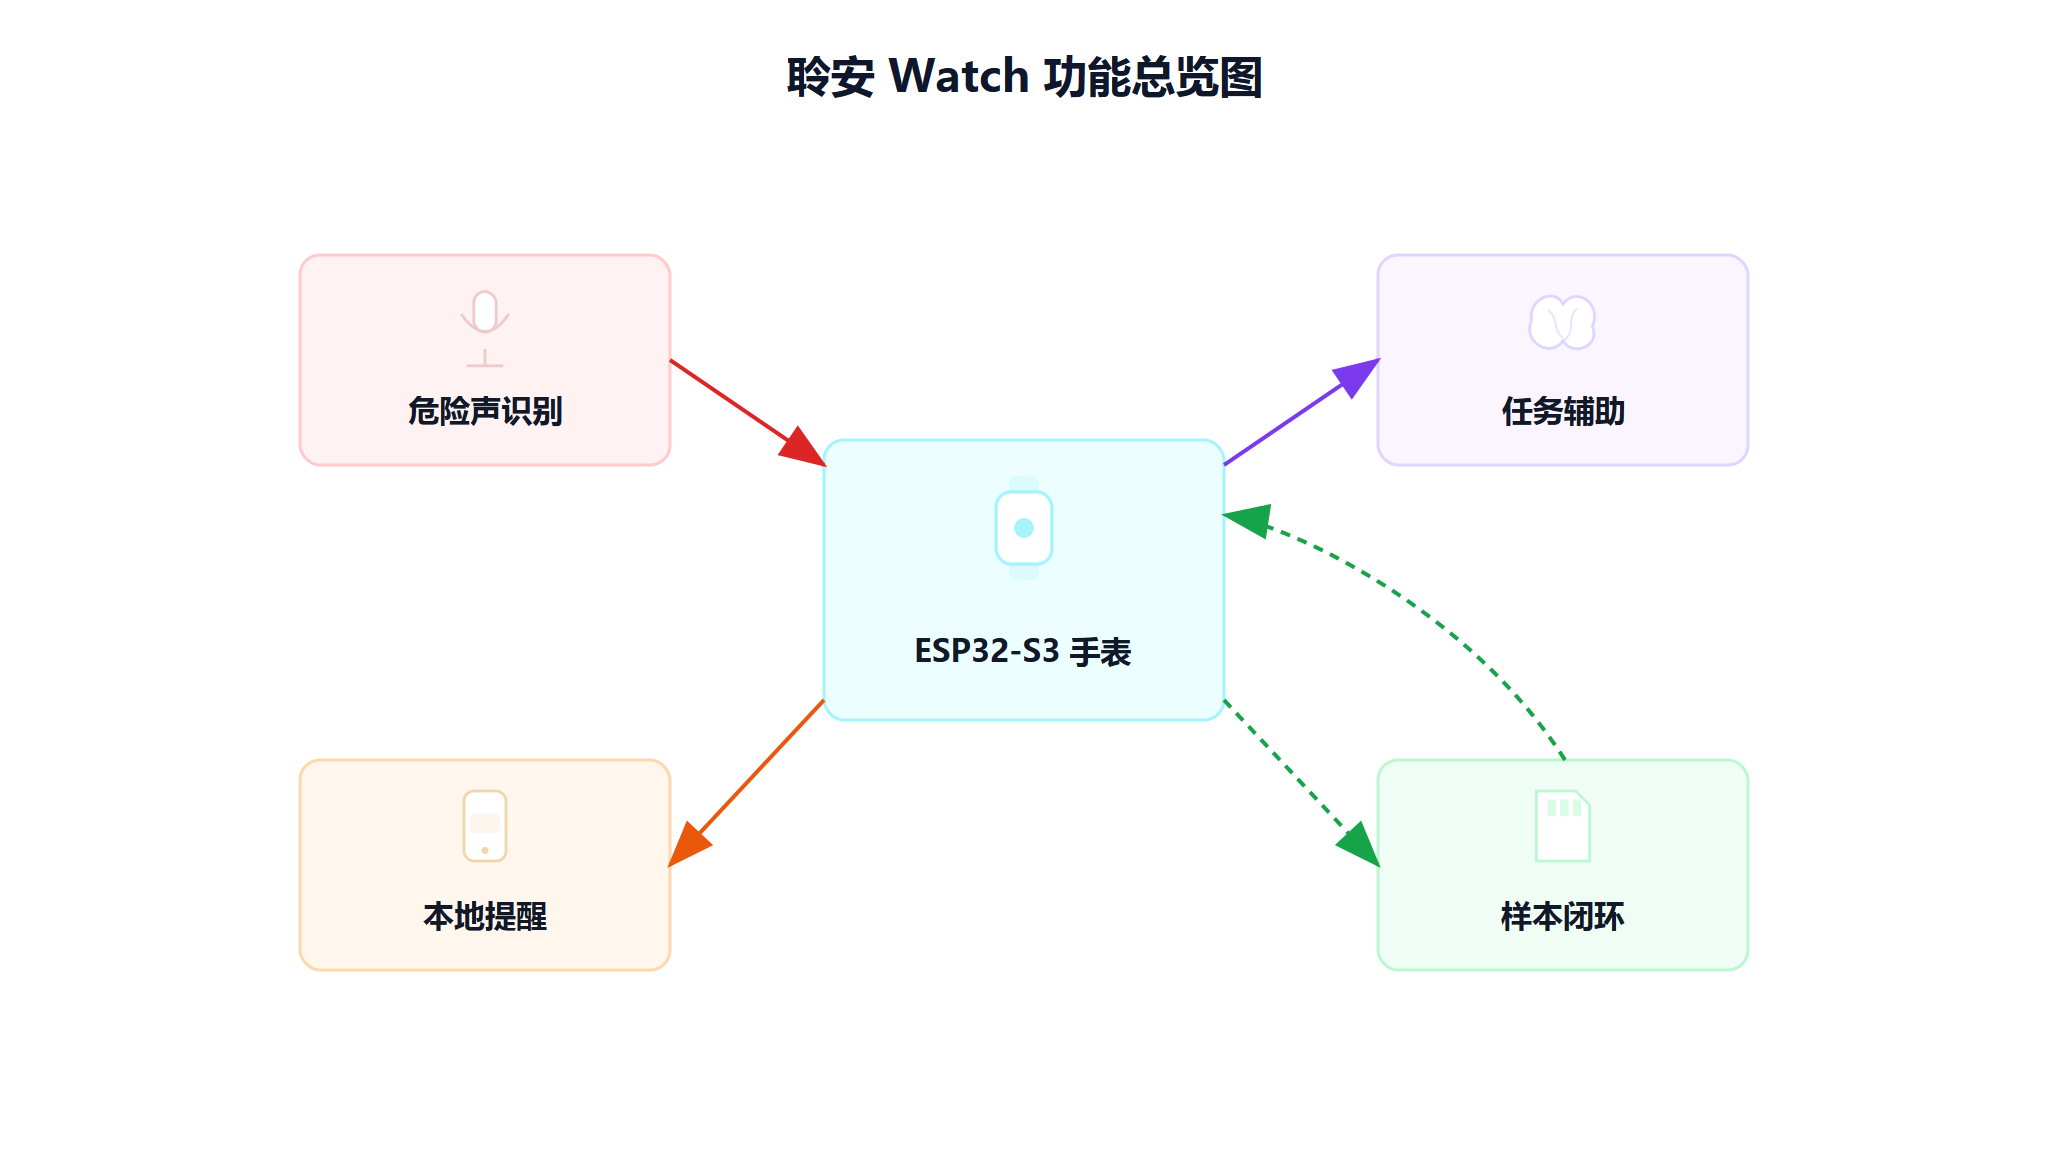
\includegraphics[width=0.95\linewidth]{figures/generated_diagrams/f00_function_overview.png}
\caption{作品功能总览图}
\end{figure}

\subsection*{1.2 应用领域}

本作品主要面向听障辅助、可穿戴设备、嵌入式边缘 AI 和 AIoT 场景。对于听障用户，交通和公共场所中的鸣笛、警笛具有较高安全价值，但用户可能无法及时获得声音线索。本作品通过端侧识别和本地提醒，将危险声学信号转化为视觉或触觉等可感知提示。在边缘 AI 方向上，声音识别、风险融合和提醒触发均部署在 ESP32-S3 手表端，使核心安全提醒不依赖云端推理链路；App/手机端远程补充告警可让用户在手机侧获知事件，后续可扩展为绑定家属或监护人的远程提醒。Hermes 任务辅助服务承担任务记录、陪伴式交互和电脑端事务协同，可扩展服务于有提醒、查询、长期记忆和跨设备操作需求的残障用户。

\begin{figure}[htbp]
\centering
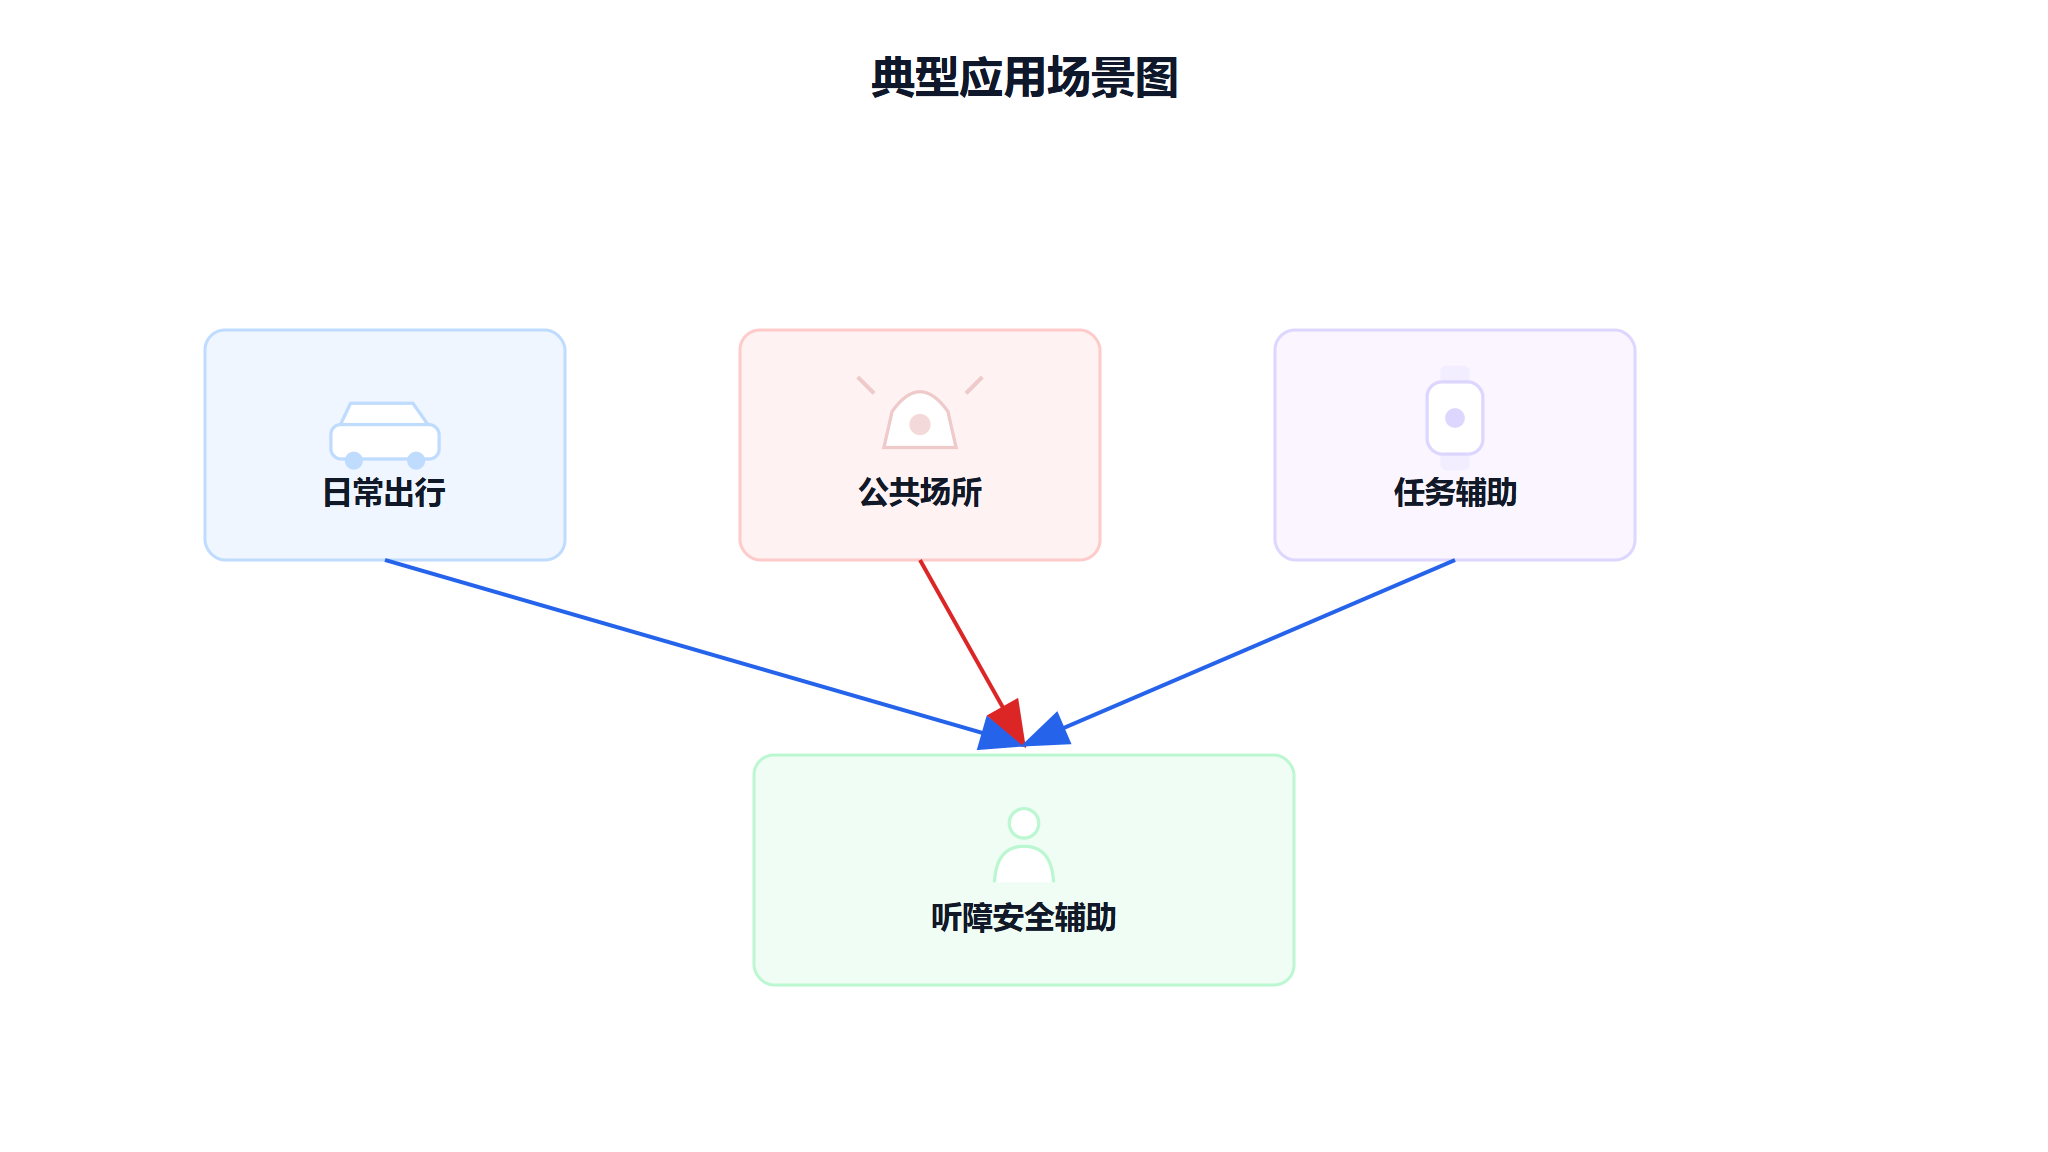
\includegraphics[width=0.95\linewidth]{figures/generated_diagrams/f00b_application_scenario.png}
\caption{典型应用场景图}
\end{figure}

\clearpage

\subsection*{1.3 主要技术特点}

\noindent\begin{tabularx}{\linewidth}{>{\bfseries}p{3.3cm}>{\RaggedRight\arraybackslash}X}
\toprule
技术特点 & 说明 \\
\midrule
ESP32-S3 部署 & 手表端承担音频采集、模型推理、状态管理、UI 展示和轻量通信。 \\
ESP-DL 推理 & 使用 Espressif 端侧深度学习能力部署 \texttt{.espdl} int8 危险声识别模型。 \\
FreeRTOS 协作 & 推理、提醒、后台发送、震动和 SD 保存由后台任务与队列协调，避免阻塞安全链路。 \\
LVGL 交互 & 用于监听状态、危险提醒、灵敏度档位和回执信息展示。 \\
风险状态机 & 通过可疑、告警、冷却等状态降低误报和抖动。 \\
灵敏度档位 & 保守/标准/敏感三档映射 0.95/0.90/0.85 单窗阈值，适配不同环境。 \\
本地提醒闭环 & 危险告警状态直接驱动高对比 UI 和 220ms--90ms--220ms 强震动作，断网时仍保持核心安全能力。 \\
后台安全监听 & 后台服务按电源预算、麦克风占用和前台运行资源调度安全监听。 \\
App 端补充告警 & 确认危险后由后台任务上报告警，云服务端转发到 App/手机端；家属或监护人绑定作为后续扩展。 \\
本地样本闭环 & 在 SD 卡保存危险触发前后 WAV 与 JSON，为模型优化提供样本依据。 \\
真机验证链路 & 通过板端日志、模型文件、状态机流转和接口联调证明核心链路可运行。 \\
Hermes 辅助 & 手表作为个人 AI Agent 随身入口，提交任务、接收回执并联动电脑端工具。 \\
\bottomrule
\end{tabularx}

\clearpage

\subsection*{1.4 主要性能与验证指标}

{\small
\noindent\begin{tabularx}{\linewidth}{p{3.2cm}>{\RaggedRight\arraybackslash}X p{3.0cm}}
\toprule
指标项 & 测试/评价口径 & 当前结果 \\
\midrule
危险声类别 & 当前模型已验证的危险声类别 & 鸣笛、警笛 \\
告警响应时间 & 从首次危险判断到进入危险告警状态 & 约 380--400 ms \\
模型离线准确率 & 131 条 edge 测试集，覆盖 background/horn/siren & 96.18\% \\
危险召回率 & 阈值 0.90 下危险样本检出能力 & 93.83\% \\
误报率 & 50 条 background 样本误触发统计 & 0.00\% \\
板端特征与推理耗时 & ESP32-S3 样例固件 3 条内置样本自检 & Fbank 32.66 ms，推理 53.41 ms \\
模型文件大小 & 当前部署 ESP-DL 模型文件 & 31.4 KB \\
内存与存储占用 & 板端 ESP-DL 运行报告 & RAM 5.6 KB；PSRAM 272.7 KB；Flash 31.4 KB \\
状态机流转 & 监听、可疑、告警、冷却状态迁移 & 已完整观测 \\
灵敏度档位 & 保守/标准/敏感三档单窗阈值 & 0.95 / 0.90 / 0.85 \\
震动提醒节奏 & 首次确认危险后的强震动作 & 220/90/220 ms \\
危险样本保存 & SD 卡保存触发前后音频与元数据 & 约 2 s WAV + JSON \\
App 远程提醒链路 & 手表告警、云服务端转发、App/手机通知栏 & 手机端链路已验证；家属绑定为后续扩展 \\
连续运行稳定性 & 默认安全监听 24 h 连续运行测试 & 无崩溃、无看门狗复位、无内存耗尽 \\
可穿戴整机参数 & 整机重量、电池容量、待机/监听功耗、连续续航时间 & 待实测数据补充 \\
\bottomrule
\end{tabularx}
}

\subsection*{1.5 主要创新点}

\begin{enumerate}
  \item 端侧危险声识别：在 ESP32-S3 手表端部署 ESP-DL int8 模型，将鸣笛、警笛等高价值危险声音的识别放在本地完成，降低网络依赖和响应延迟。
  \item 本地风险状态机与震动提醒：通过连续确认、告警保持和冷却抑制把模型输出转化为稳定风险状态，并用高对比界面和短促强震形成听障用户可感知的本地闭环。
  \item App 端远程补充告警：危险确认后先触发手表本地提醒，再由后台任务上报云服务端并转发到 App/手机通知栏，为用户远程获知和后续家属/监护人绑定提醒预留工程边界。
  \item SD 本地样本闭环：在危险事件触发时保存前后短音频和 JSON 元数据，支撑人工复盘、误报分析、离线标注和后续模型优化。
\end{enumerate}

\subsection*{1.6 设计流程}

本作品的设计流程为：首先分析听障用户在公共场所和交通环境中的危险声音感知需求；然后确定 ESP32-S3 手表端的音频采集、ESP-DL 推理、风险融合和本地提醒主链路；接着实现灵敏度档位、震动提醒、低功耗安全监听、App/手机端远程补充告警、SD 样本保存和 LVGL 状态展示；随后通过板端日志、模型文件、状态机流转和接口联调验证核心功能；最后将 Hermes 作为面向残障用户的任务记录、回执接收和电脑端事务协同入口接入云服务端，并根据误报、资源占用和真机体验继续优化。

\begin{figure}[htbp]
\centering
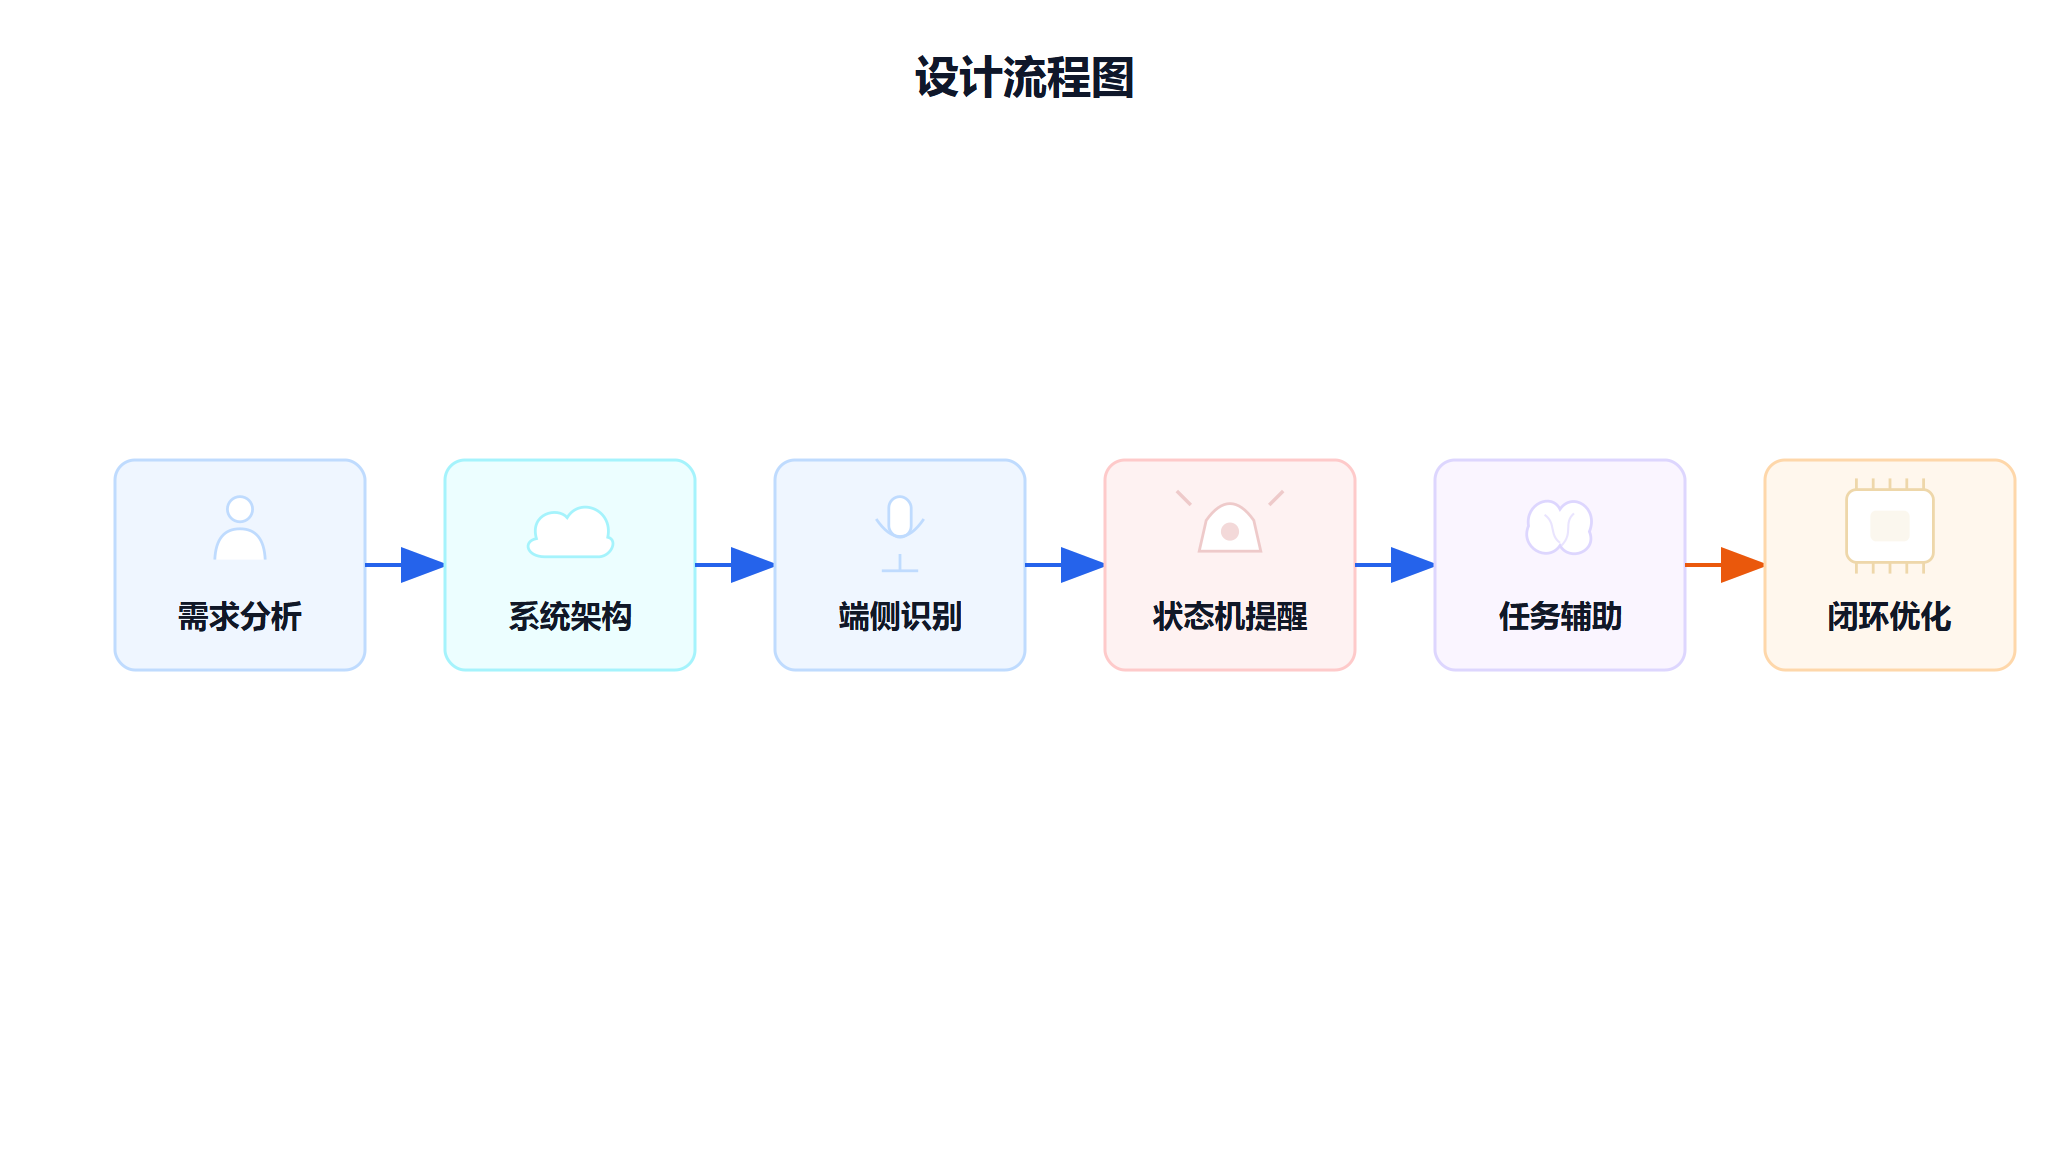
\includegraphics[width=0.95\linewidth]{figures/generated_diagrams/f00c_design_process.png}
\caption{设计流程图}
\end{figure}

\section*{第二部分\quad 系统组成及功能说明}
\addcontentsline{toc}{section}{第二部分 系统组成及功能说明}

本部分从整体架构、硬件组成、软件组成、边缘 AI 识别流程、风险状态机、数据闭环和辅助协同接口等方面阐述系统设计细节。

\subsection*{2.1 整体介绍}

系统以 ESP32-S3 手表端为核心，由手表端本地安全链路、后台安全监听链路、App/云服务端远程补充告警链路和辅助交互链路组成。手表端负责环境音采集、ESP-DL 推理、风险状态机、灵敏度档位、本地提醒和危险样本缓存；后台服务管理器负责把用户安全监听开关、电源预算、麦克风占用和前台运行资源统一转化为危险识别会话的启动、暂停和恢复策略；云服务端负责设备鉴权、危险告警接收、请求去重、超时控制和辅助任务转接；App/手机通知端用于远程补充提醒，后续可扩展为绑定家属或监护人提醒。危险声音链路从环境声音进入手表端麦克风，经端侧特征处理、ESP-DL 推理和风险状态机后立即触发屏幕与震动提醒，随后由后台任务异步上报告警并在 SD 卡保存短音频样本。Hermes 位于辅助交互链路，用于处理用户主动发起的任务记录、提醒创建、信息查询、回执接收和授权范围内的电脑端事务协同，使手表在安全提醒之外也具备随身任务辅助能力。

\begin{figure}[htbp]
\centering
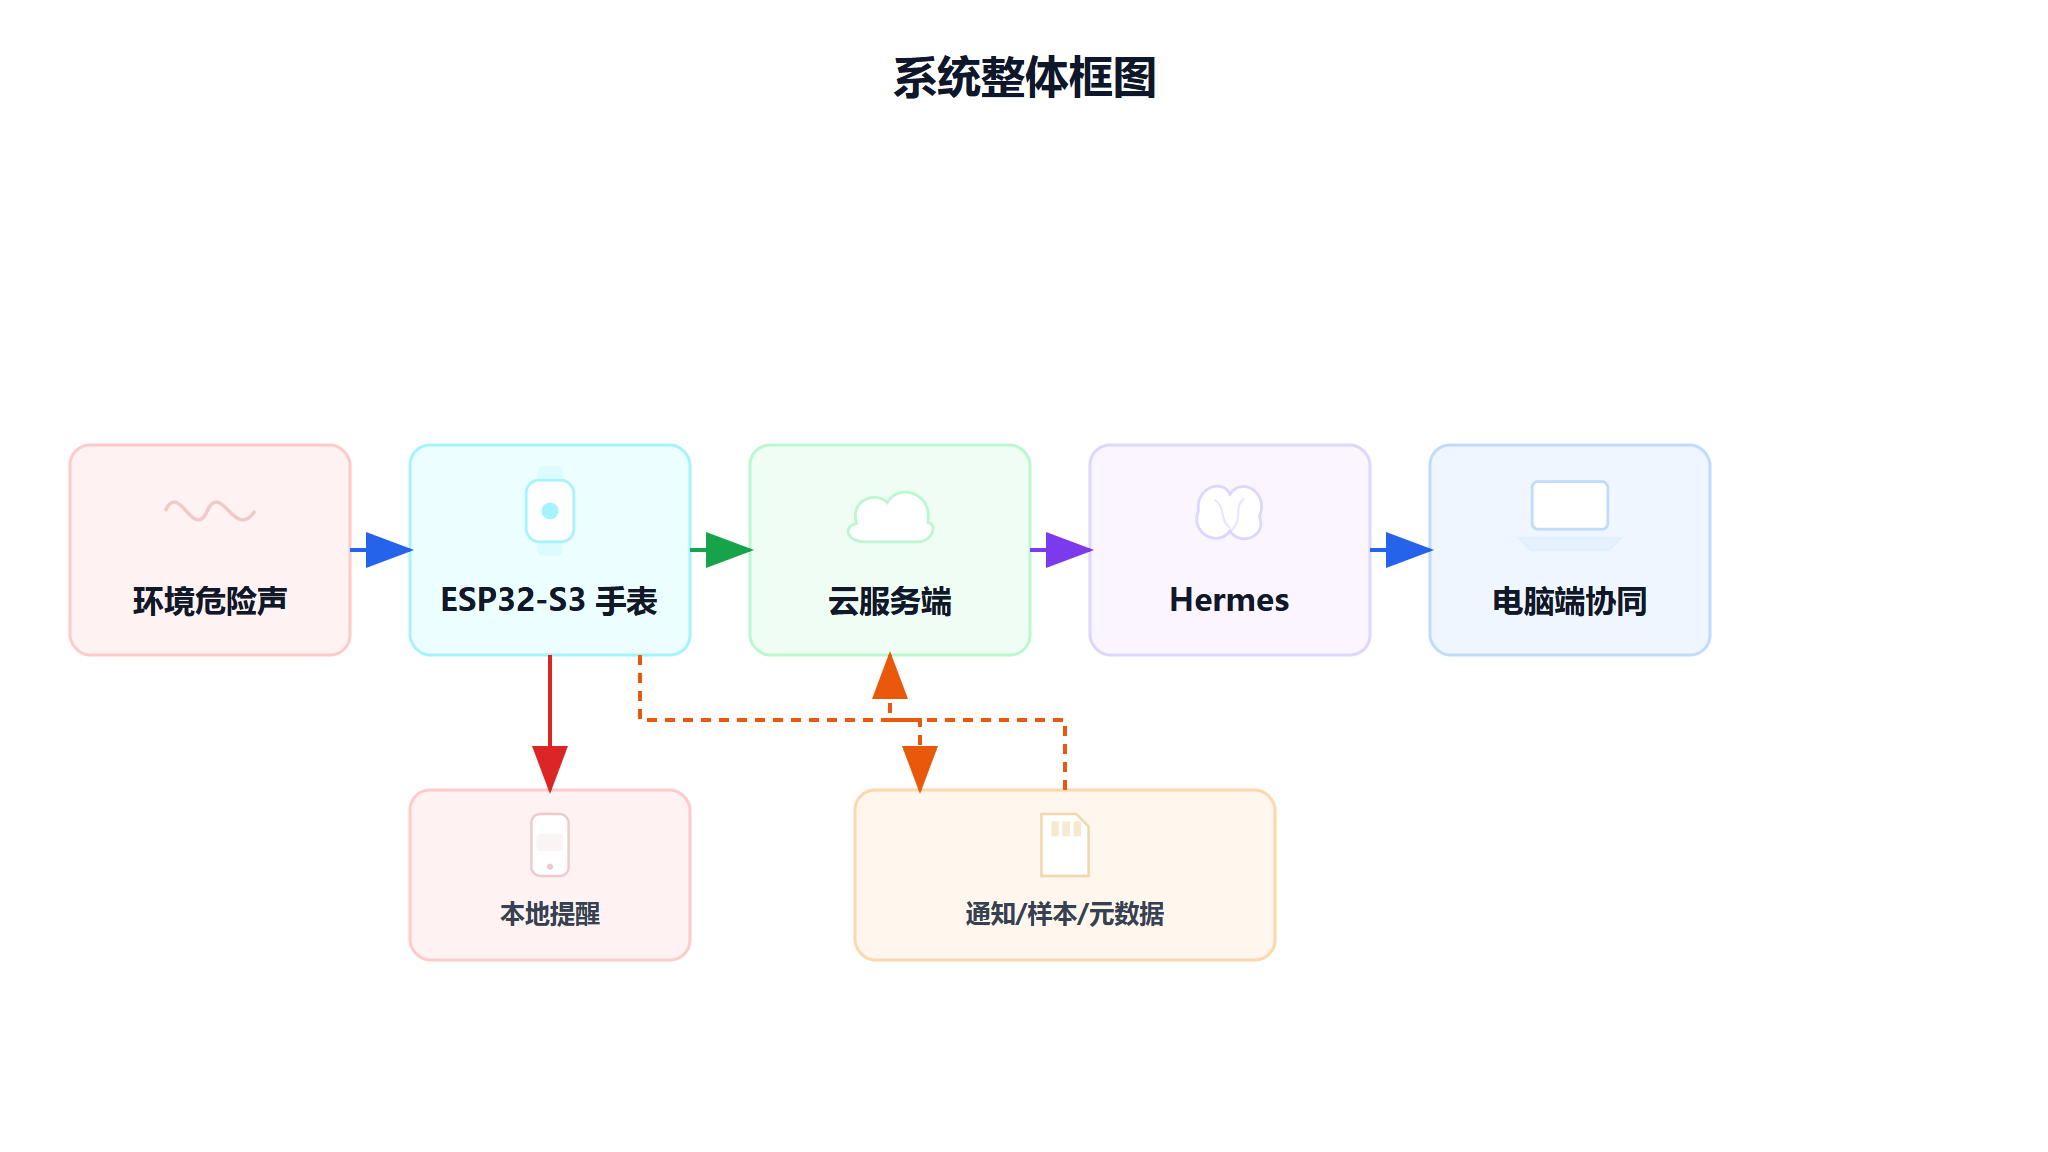
\includegraphics[width=0.95\linewidth]{figures/generated_diagrams/f01_system_architecture.png}
\caption{系统整体框图}
\end{figure}

\subsection*{2.2 硬件系统介绍}

\subsubsection*{2.2.1 硬件整体介绍}

本作品硬件系统以乐鑫 ESP32-S3R8 为主控，外围电路围绕可穿戴终端的音频采集、端侧推理、显示触摸、电源管理、提醒输出和本地存储展开。系统通过 USB Type-C 接口供电与调试，使用 AXP2101 进行多路电源管理，板载 QMI8658C 六轴 IMU 与 PCF85063AT RTC；音频部分集成双 MEMS 麦克风、ES7210 ADC、ES8311 编解码器与 NS4150B D 类功放，并通过 DS2413 控制马达振动；显示部分通过 FPC 接口连接 AMOLED 显示屏与触摸屏，同时预留 SD 卡与 SIM 卡接口。该硬件结构能够支撑危险声音采集、ESP-DL 端侧推理、高对比屏幕提醒、震动提醒、SD 本地样本保存和后续通信扩展。

\begin{figure}[htbp]
\centering
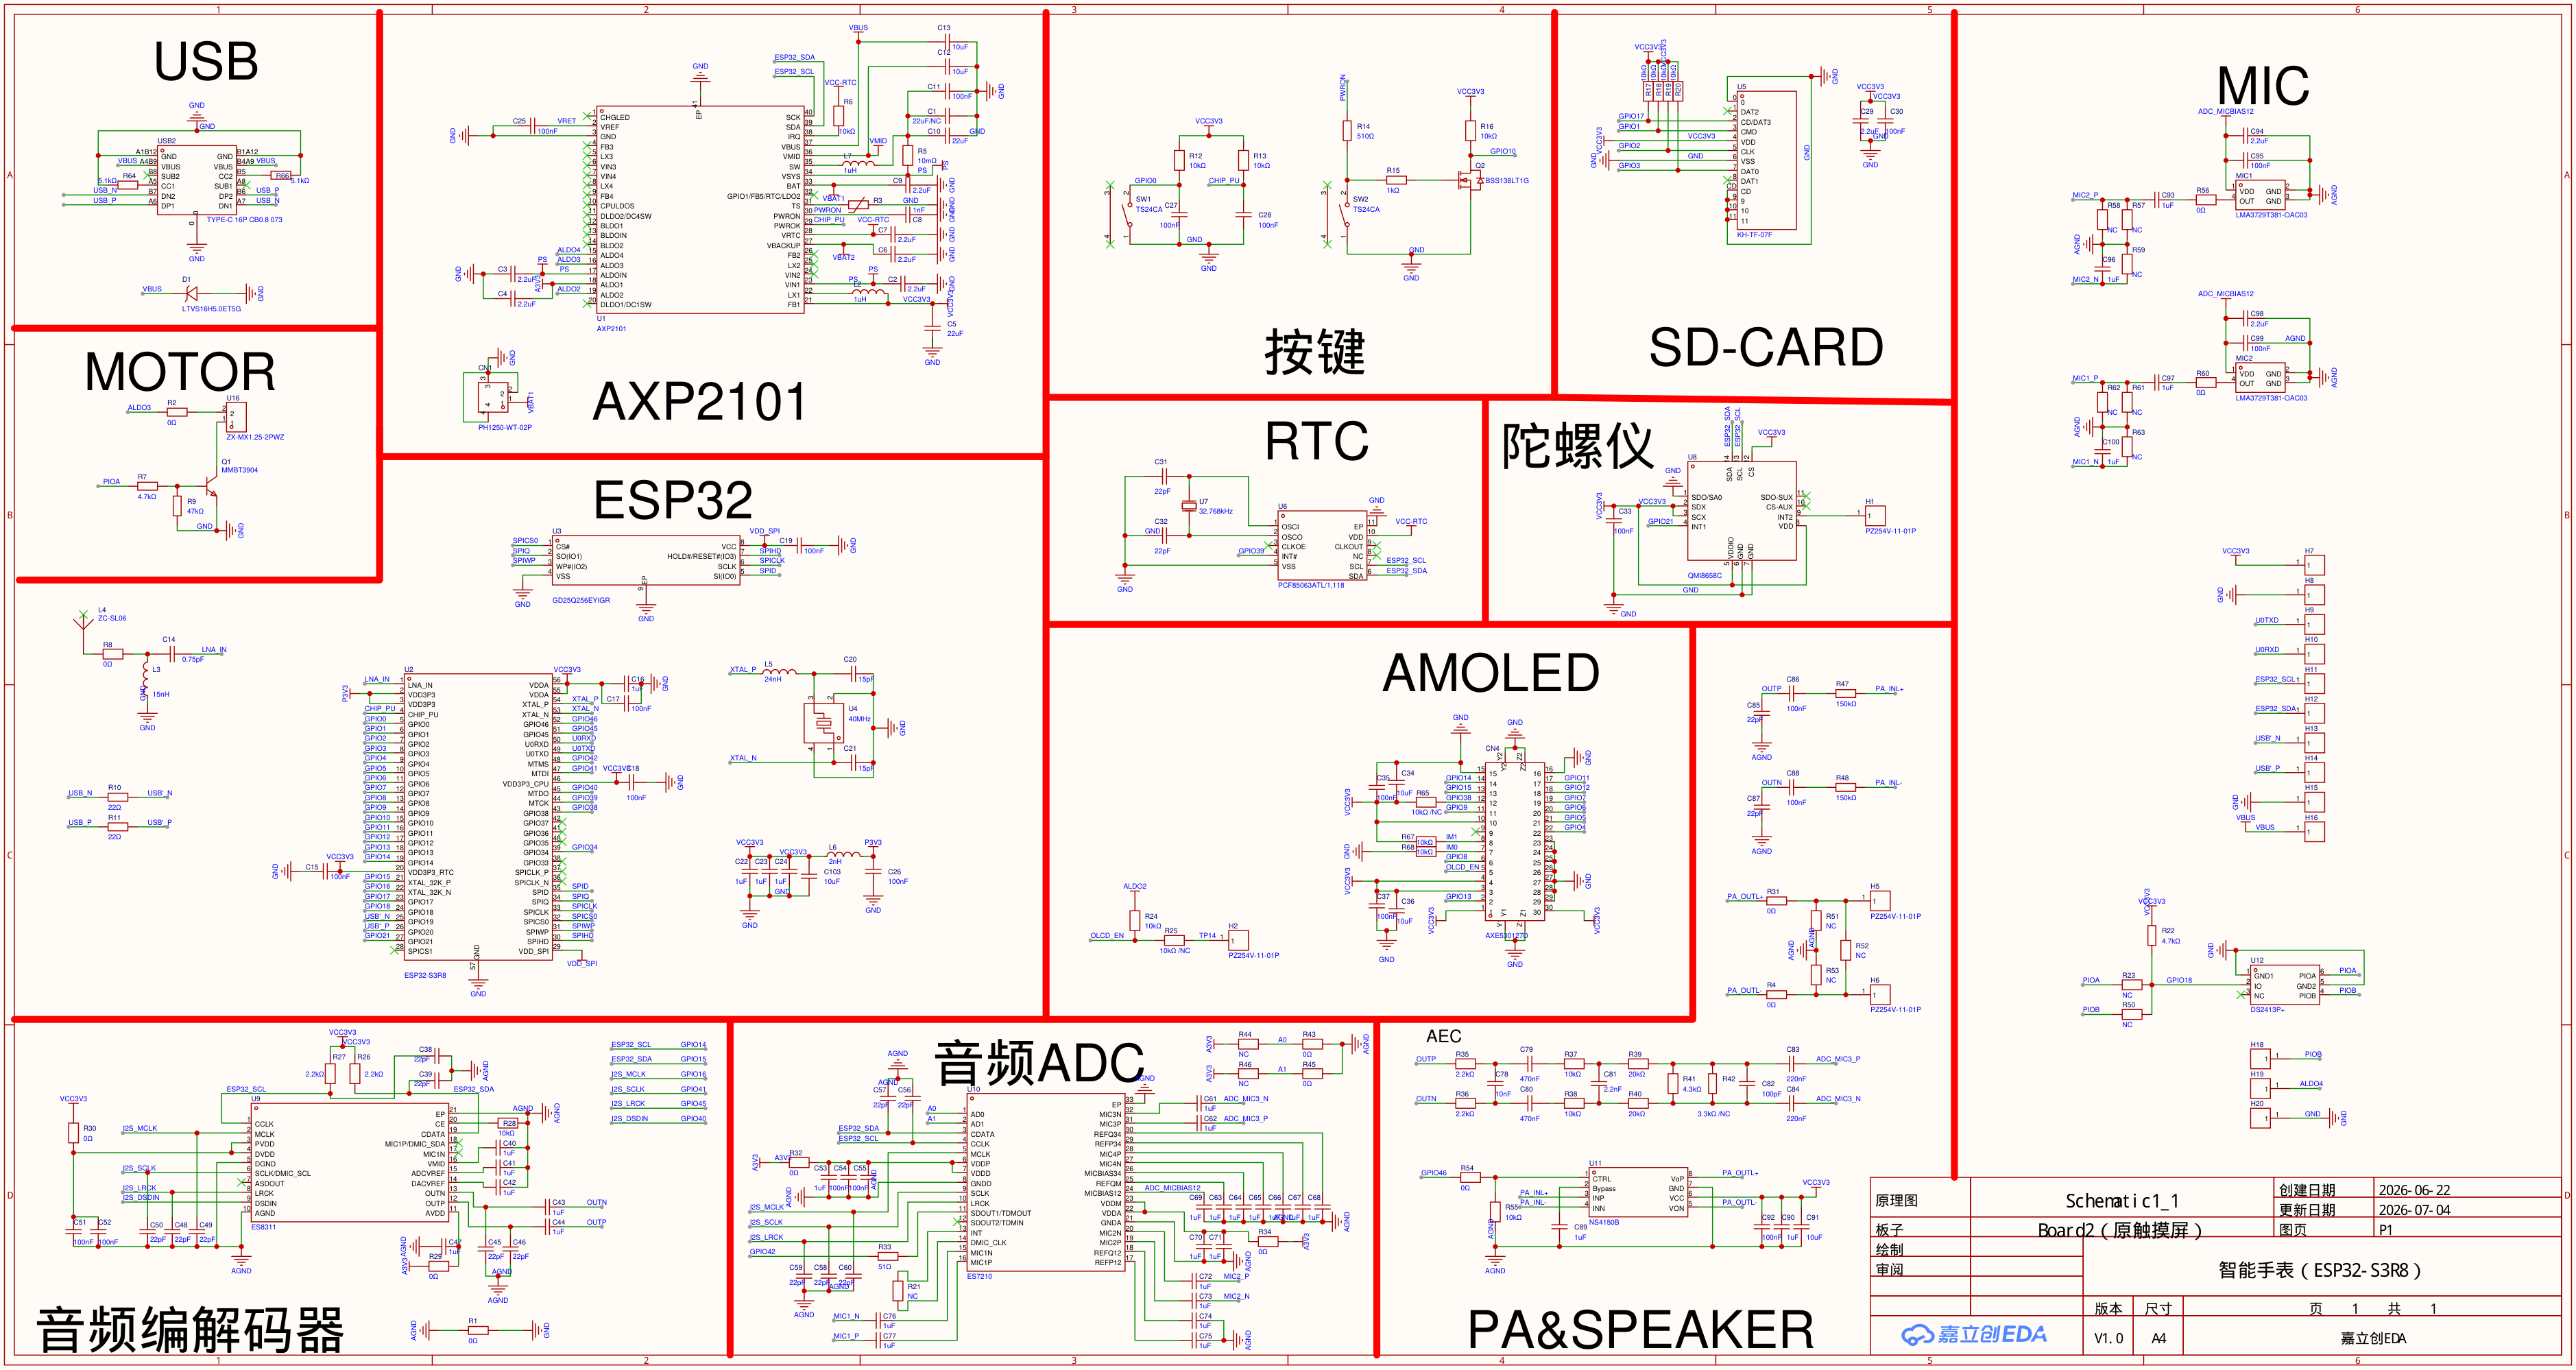
\includegraphics[width=\linewidth]{figures/hardware/f13_system_schematic.png}
\caption{系统完整原理图}
\label{fig:system-schematic}
\end{figure}

整机实物照片作为最终工程证据，集中放在第三部分成果验证中展示，避免与本节硬件设计图重复。

\subsubsection*{2.2.2 机械设计介绍}

PCB 板框尺寸为 46.0 mm $\times$ 37.0 mm，采用四层板设计。板上预留 5 个 $\Phi$1.8 mm 定位孔用于外壳装配，顶部设有 USB Type-C 矩形避让口，左右两侧采用圆角造型，与手表外形和佩戴结构相匹配，便于嵌入表壳。该机械边界为屏幕、麦克风、触摸输入、马达提醒和电池/接口区域预留了基本装配空间；后续实物证明以整机正面、斜 45 度和佩戴/装配状态组图为准。

\begin{figure}[htbp]
\centering
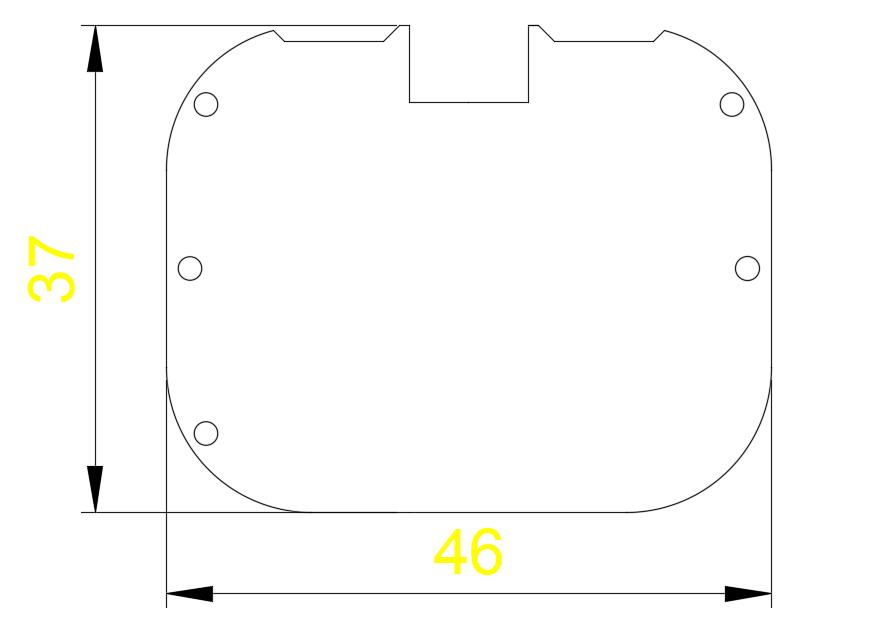
\includegraphics[width=0.7\linewidth]{figures/hardware/f14_pcb_outline.png}
\caption{PCB 板框图}
\label{fig:pcb-outline}
\end{figure}

\subsubsection*{2.2.3 电路各模块介绍}

电路设计围绕主控、音频、电源、显示触摸和扩展接口展开，各模块与端侧 AI 安全提醒链路的关系如下表所示。电源管理模块保证手表长期运行的供电基础；双麦克风与音频 ADC 为危险声识别提供输入；AMOLED 与触摸屏承担告警显示和用户交互；马达与扬声器用于补充触觉/声音提醒；SD 卡接口用于本地样本保存。

\clearpage

\begin{center}
\textbf{表 1：硬件电路模块说明}
\end{center}
\noindent
\begin{tabularx}{\linewidth}{p{2.7cm}>{\RaggedRight\arraybackslash}X>{\RaggedRight\arraybackslash}p{4.6cm}}
\toprule
模块 & 设计内容 & 与作品功能的关系 \\
\midrule
电源管理 & AXP2101 PMIC 通过 I\textsuperscript{2}C 受主控管理，输入 USB 5V，输出 3.3V、1.8V、0.9V 等多路电压，并支持电池充放电管理。 & 为 ESP32-S3、音频、显示触摸、传感器和存储模块提供稳定电源，是后台安全监听和持续监听的硬件基础。 \\
主控模块 & ESP32-S3R8 外接 40 MHz 主晶振与 32.768 kHz RTC 晶振，射频端经匹配网络连接 2.4G 贴片天线，支持 Wi-Fi/BLE 双模通信。 & 承担 ESP-IDF 固件运行、ESP-DL 推理、LVGL UI、联网告警和 Hermes 云服务通信。 \\
传感器模块 & QMI8658C 六轴 IMU 通过 I\textsuperscript{2}C 与主控通信，PCF85063AT RTC 提供独立时间基准。 & IMU 可用于佩戴/运动状态扩展，RTC 为事件记录、样本元数据和低功耗运行提供时间基础。 \\
音频模块 & 双 MEMS 麦克风经 ES7210 ADC 转为数字音频，ES8311 编解码器与 NS4150B D 类功放负责音频输出，DS2413 控制马达振动。 & 支撑环境危险声采集、用户语音输入、提醒声音输出和听障场景下的震动提醒。 \\
显示触摸 & 通过 30Pin 0.4 mm FPC 连接 AMOLED 屏，显示数据经 SPI/MIPI 传输，触摸控制器通过 I\textsuperscript{2}C 上报坐标。 & 展示监听状态、危险告警、灵敏度档位、App 告警回执和 Hermes 任务辅助回执。 \\
通信存储 & USB Type-C 用于供电与调试，SD 卡座支持外部存储扩展，SIM 卡座预留蜂窝通信，GD25Q256E SPI Flash 用于固件与资源文件。 & 支撑调试烧录、SD 本地样本保存、后续联网扩展和固件/资源存储。 \\
\bottomrule
\end{tabularx}

\clearpage

\begin{center}
\begin{minipage}{0.48\linewidth}
  \centering
  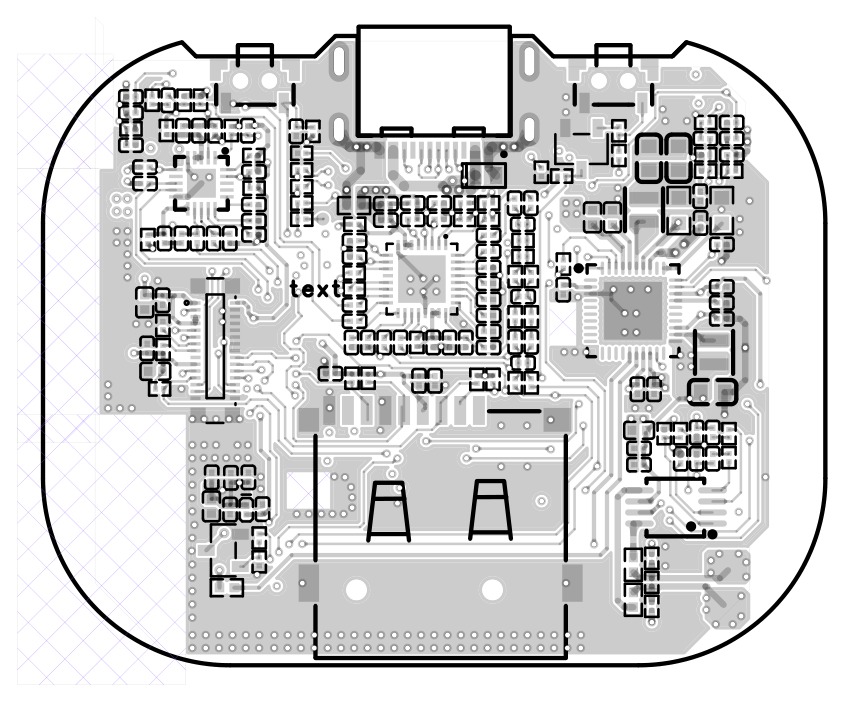
\includegraphics[width=\linewidth]{figures/hardware/f15_pcb_top_layout.png}\\
  {\small PCB 顶层布局}
\end{minipage}\hfill
\begin{minipage}{0.48\linewidth}
  \centering
  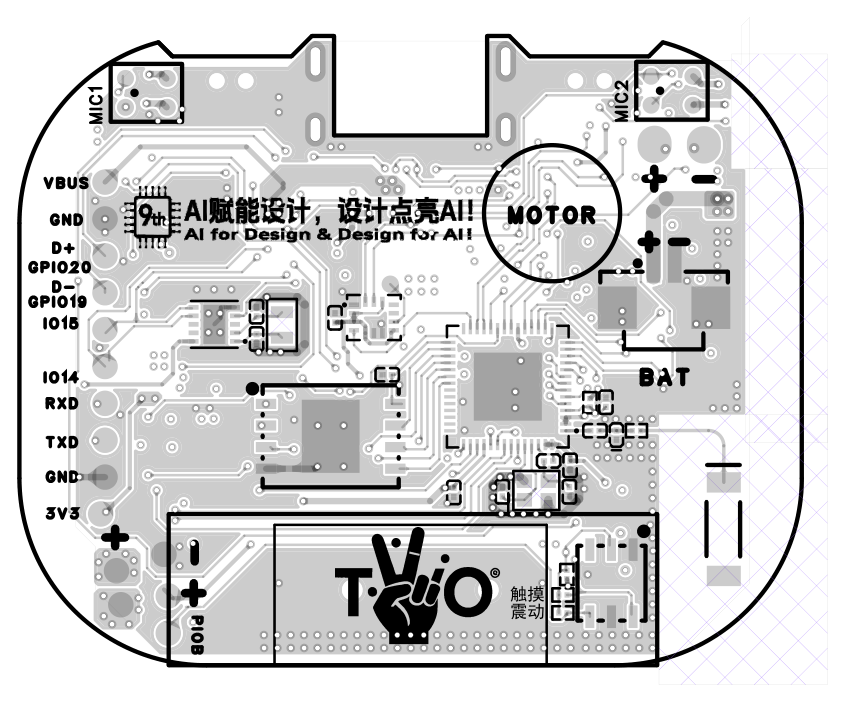
\includegraphics[width=\linewidth]{figures/hardware/f16_pcb_bottom_layout.png}\\
  {\small PCB 底层布局}
\end{minipage}
\par\vspace{0.8em}
\refstepcounter{figure}
\label{fig:pcb-layout}
图 \thefigure：PCB 顶层与底层布局图
\end{center}

\clearpage

\subsection*{2.3 软件系统介绍}

\subsubsection*{2.3.1 软件整体介绍}

软件系统分为手表端固件和服务器端服务两部分。手表端基于 ESP-IDF 组织工程，核心职责是 UI、音频采集、模型推理、风险融合、灵敏度档位、提醒管理、后台安全监听、告警投递和 SD 样本缓存；Hermes 页面状态属于辅助交互模块。云服务端作为 ESP32-S3 与 App/手机端、Hermes 服务之间的桥接层，负责设备鉴权、危险告警接收、请求去重、超时控制、ASR/Hermes 转接和结构化回执。

\begin{figure}[htbp]
\centering
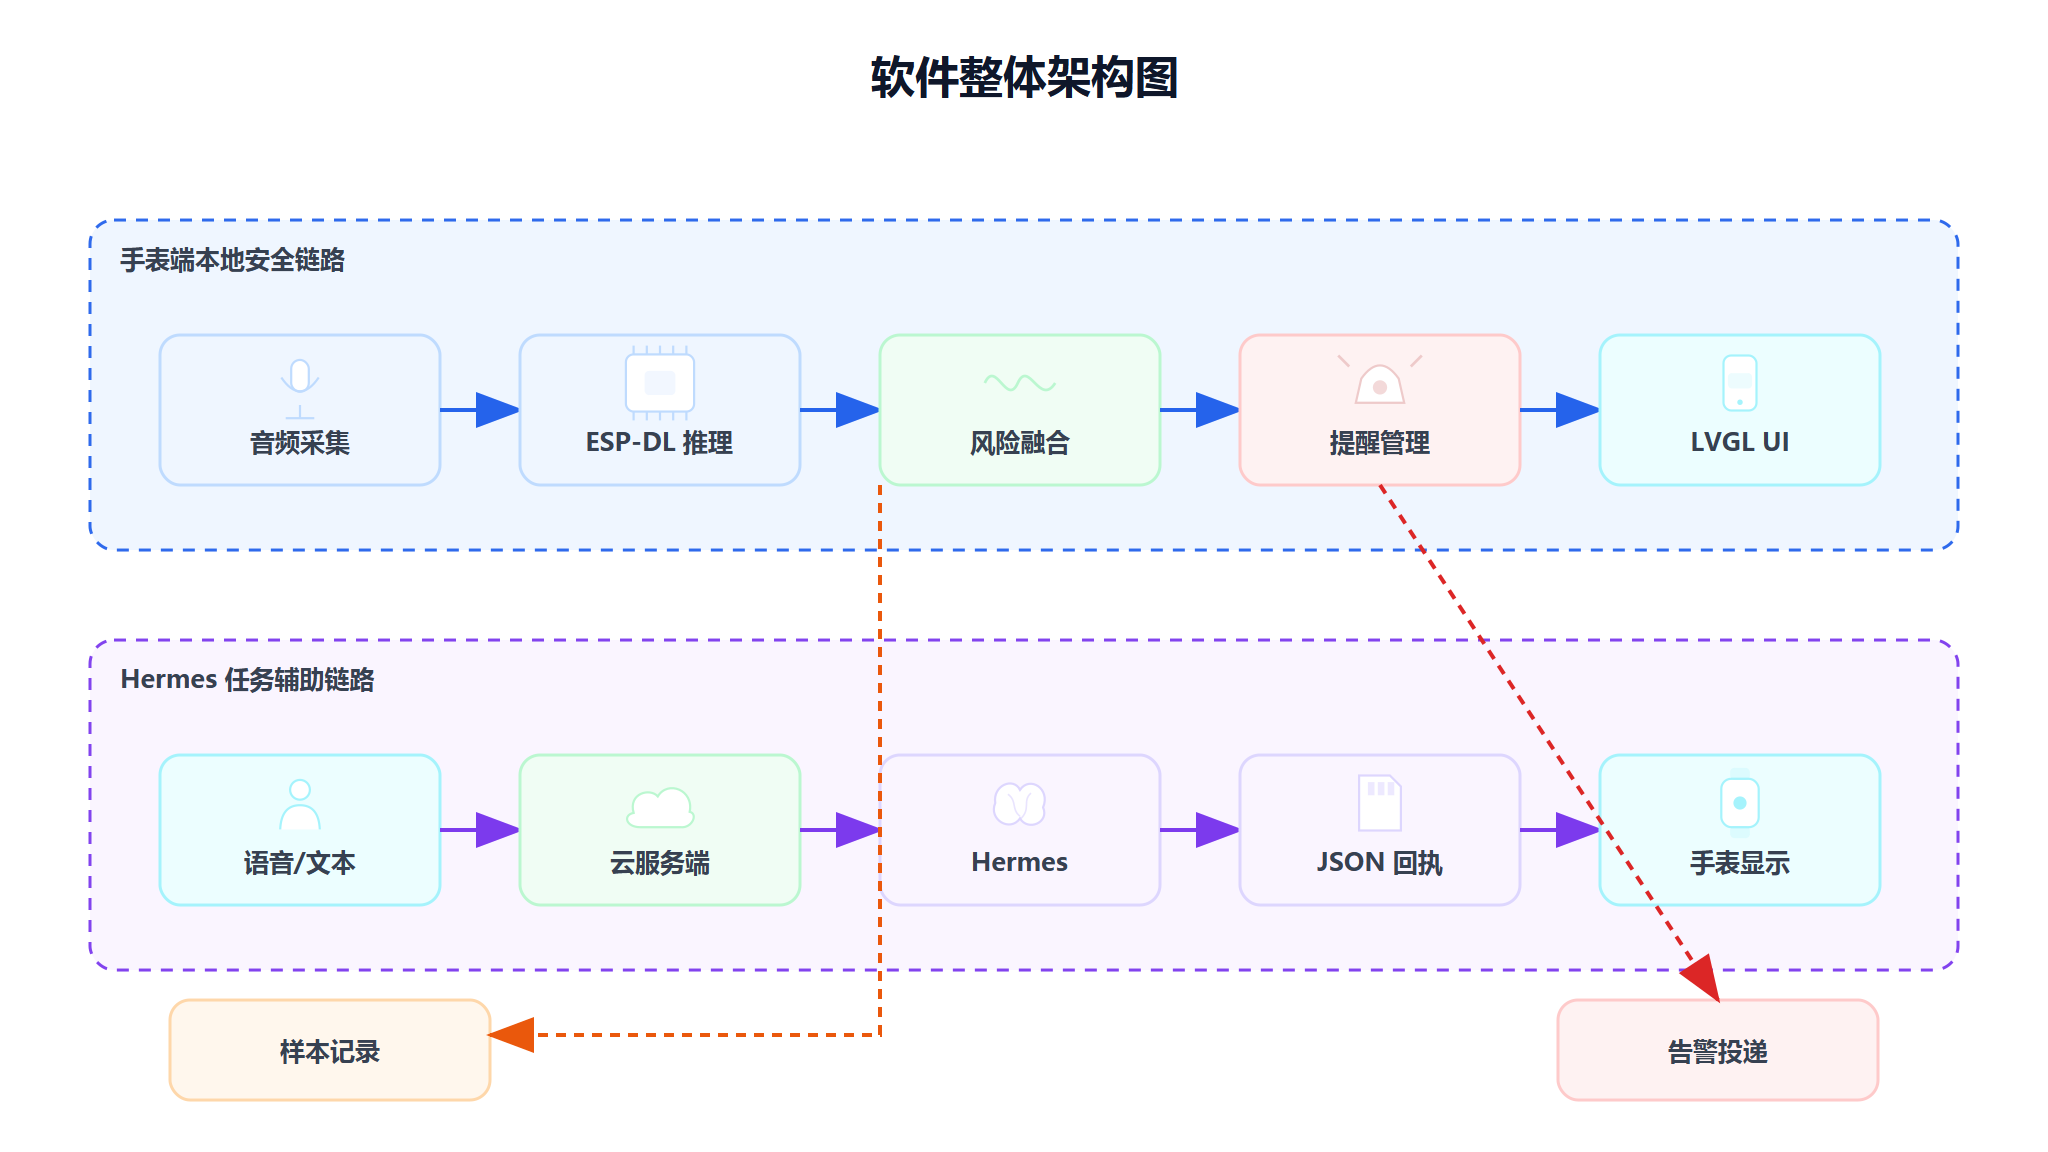
\includegraphics[width=0.95\linewidth]{figures/generated_diagrams/f02_software_architecture.png}
\caption{软件整体架构图}
\end{figure}

\subsubsection*{2.3.2 软件各模块介绍}

\noindent\begin{longtable}{>{\raggedright\arraybackslash}p{3.2cm}>{\RaggedRight\arraybackslash}p{3.6cm}>{\RaggedRight\arraybackslash}p{2.6cm}>{\RaggedRight\arraybackslash}p{2.6cm}}
\toprule
模块 & 职责 & 输入 & 输出 \\
\midrule
UI 显示层 & 优先展示监听、危险提醒和告警状态，辅助展示任务回执 & 状态快照、触摸/按键 & 页面显示和用户命令 \\
音频采集层 & 管理麦克风输入和音频资源 & 麦克风音频 & PCM 音频流 \\
端侧推理层 & 执行音频滑窗、特征处理和 ESP-DL 推理 & PCM 音频窗口 & 模型输出 \\
风险融合服务 & 将单窗模型输出融合为稳定风险状态 & 危险概率/标签 & 风险状态快照 \\
灵敏度策略 & 将保守/标准/敏感档位映射为单窗阈值和后处理参数组 & 用户档位 & ESP-DL 阈值与状态机参数 \\
提醒管理服务 & 触发用户提醒和危险提示 & 告警状态 & 屏幕/震动/音频提醒动作 \\
后台安全监听 & 按用户开关、电源预算和资源占用维护后台危险识别会话 & 监听开关、资源状态 & 会话启停与恢复 \\
样本记录服务 & 缓存连续音频，并在危险触发后保存 WAV/JSON & 本地音频片段与触发事件 & SD 卡样本文件 \\
告警投递服务 & 将危险事件异步提交到云服务端 & 危险告警事件 & App 远程提醒链路输入 \\
辅助交互页面服务 & 维护 Hermes 页面命令、状态快照和回执 & UI 命令、云端回执 & 辅助页面状态 \\
辅助请求客户端 & 提交语音或文本请求到云服务端 & 录音/文本、设备状态 & 结构化响应 \\
云服务端 & 设备鉴权、危险告警接收和辅助任务转接 & 手表请求 & 通知事件与结构化回执 \\
\bottomrule
\end{longtable}

\noindent\textbf{端侧危险声识别流程。}

危险声识别是保障听障用户安全的第一道防线，其设计需兼顾实时性、准确性和资源约束三方面。与依赖远程判断再等待结果的方案相比，端侧推理在延迟（板端样例固件中特征提取与推理合计约 86 ms）、隐私和离线可用性（断网仍可本地提醒）上具有不可替代的优势。ESP32-S3 内置的向量指令加速和 ESP-DL 提供的轻量化模型部署能力，使得在可穿戴资源预算内运行危险声分类成为可能。

本系统当前优先识别两类对听障用户出行安全影响最大的危险声：鸣笛（车辆近距离接近）和警笛（紧急车辆通行）。这两类声音的共同特征是频谱能量集中、持续时间长、声学模式稳定，适合用轻量卷积模型从短时音频窗口中区分。模型训练与离线评估在 PC 端基于 AudioClassification-Pytorch 和 PyTorch 完成，CUDA 仅作为训练/评估加速环境；端侧部署时将稳定模型导出为 ESP-DL 可加载的 \texttt{.espdl} 格式，在 ESP32-S3 上进行 int8 推理。

危险声识别流程为：麦克风采集后进入音频重采样与滑动窗口处理，生成 Fbank 等特征表示，再由 ESP-DL 模型推理得到危险/安全输出。随后风险融合层根据当前灵敏度档位进行连续窗口确认、告警保持和冷却处理，最终由提醒层转化为屏幕或震动等用户可感知反馈。

\begin{figure}[htbp]
\centering
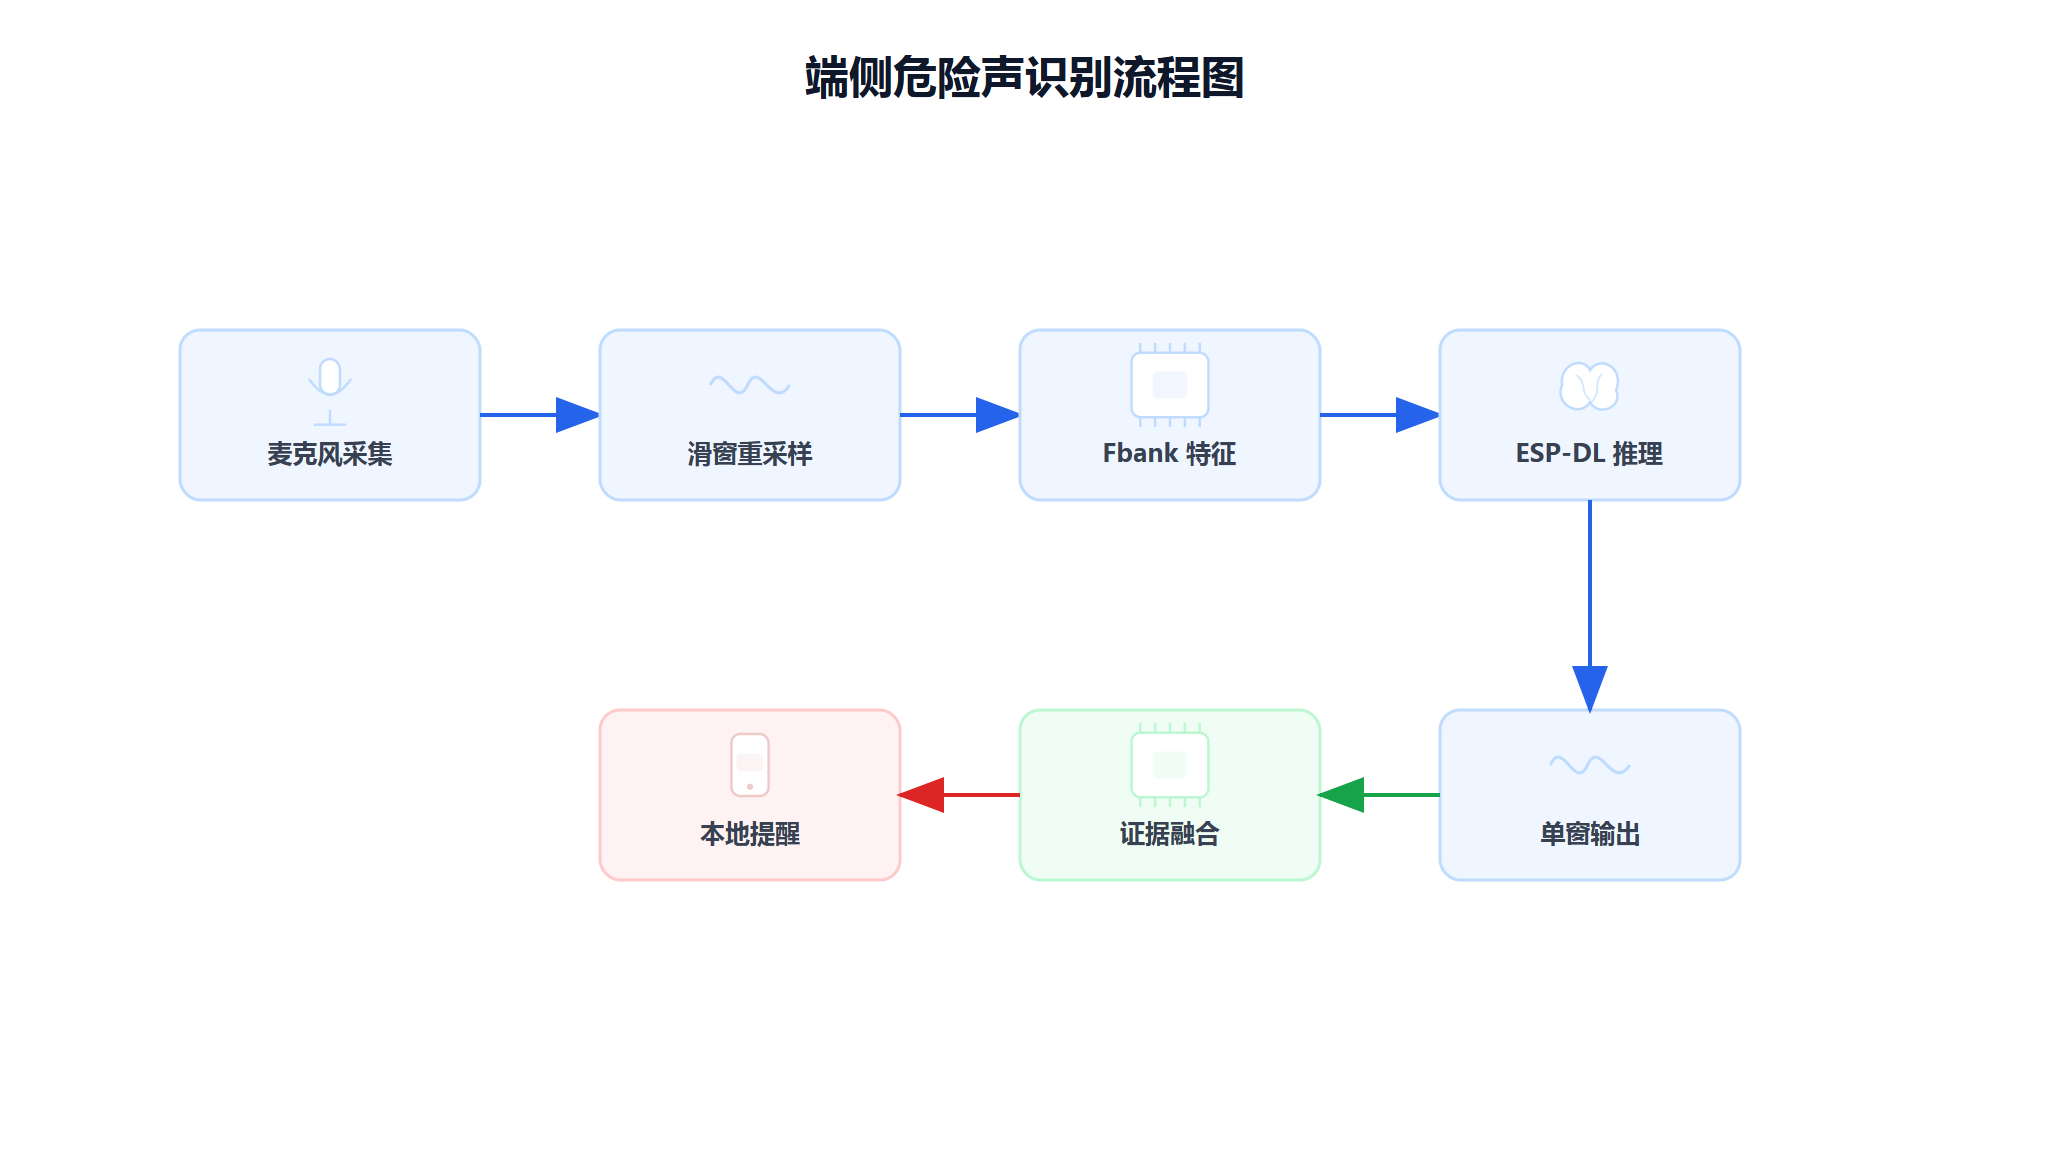
\includegraphics[width=0.95\linewidth]{figures/generated_diagrams/f03_edge_ai_flow.png}
\caption{端侧危险声识别流程图}
\end{figure}

\noindent\textbf{风险状态机设计。}

风险状态机用于把单窗模型结果转换为稳定的产品状态。系统默认不把一次危险输出直接等同为危险事件，而是经过连续证据确认、最短告警保持和冷却抑制，减少普通噪声或短促误判造成的打扰。

\begin{figure}[htbp]
\centering
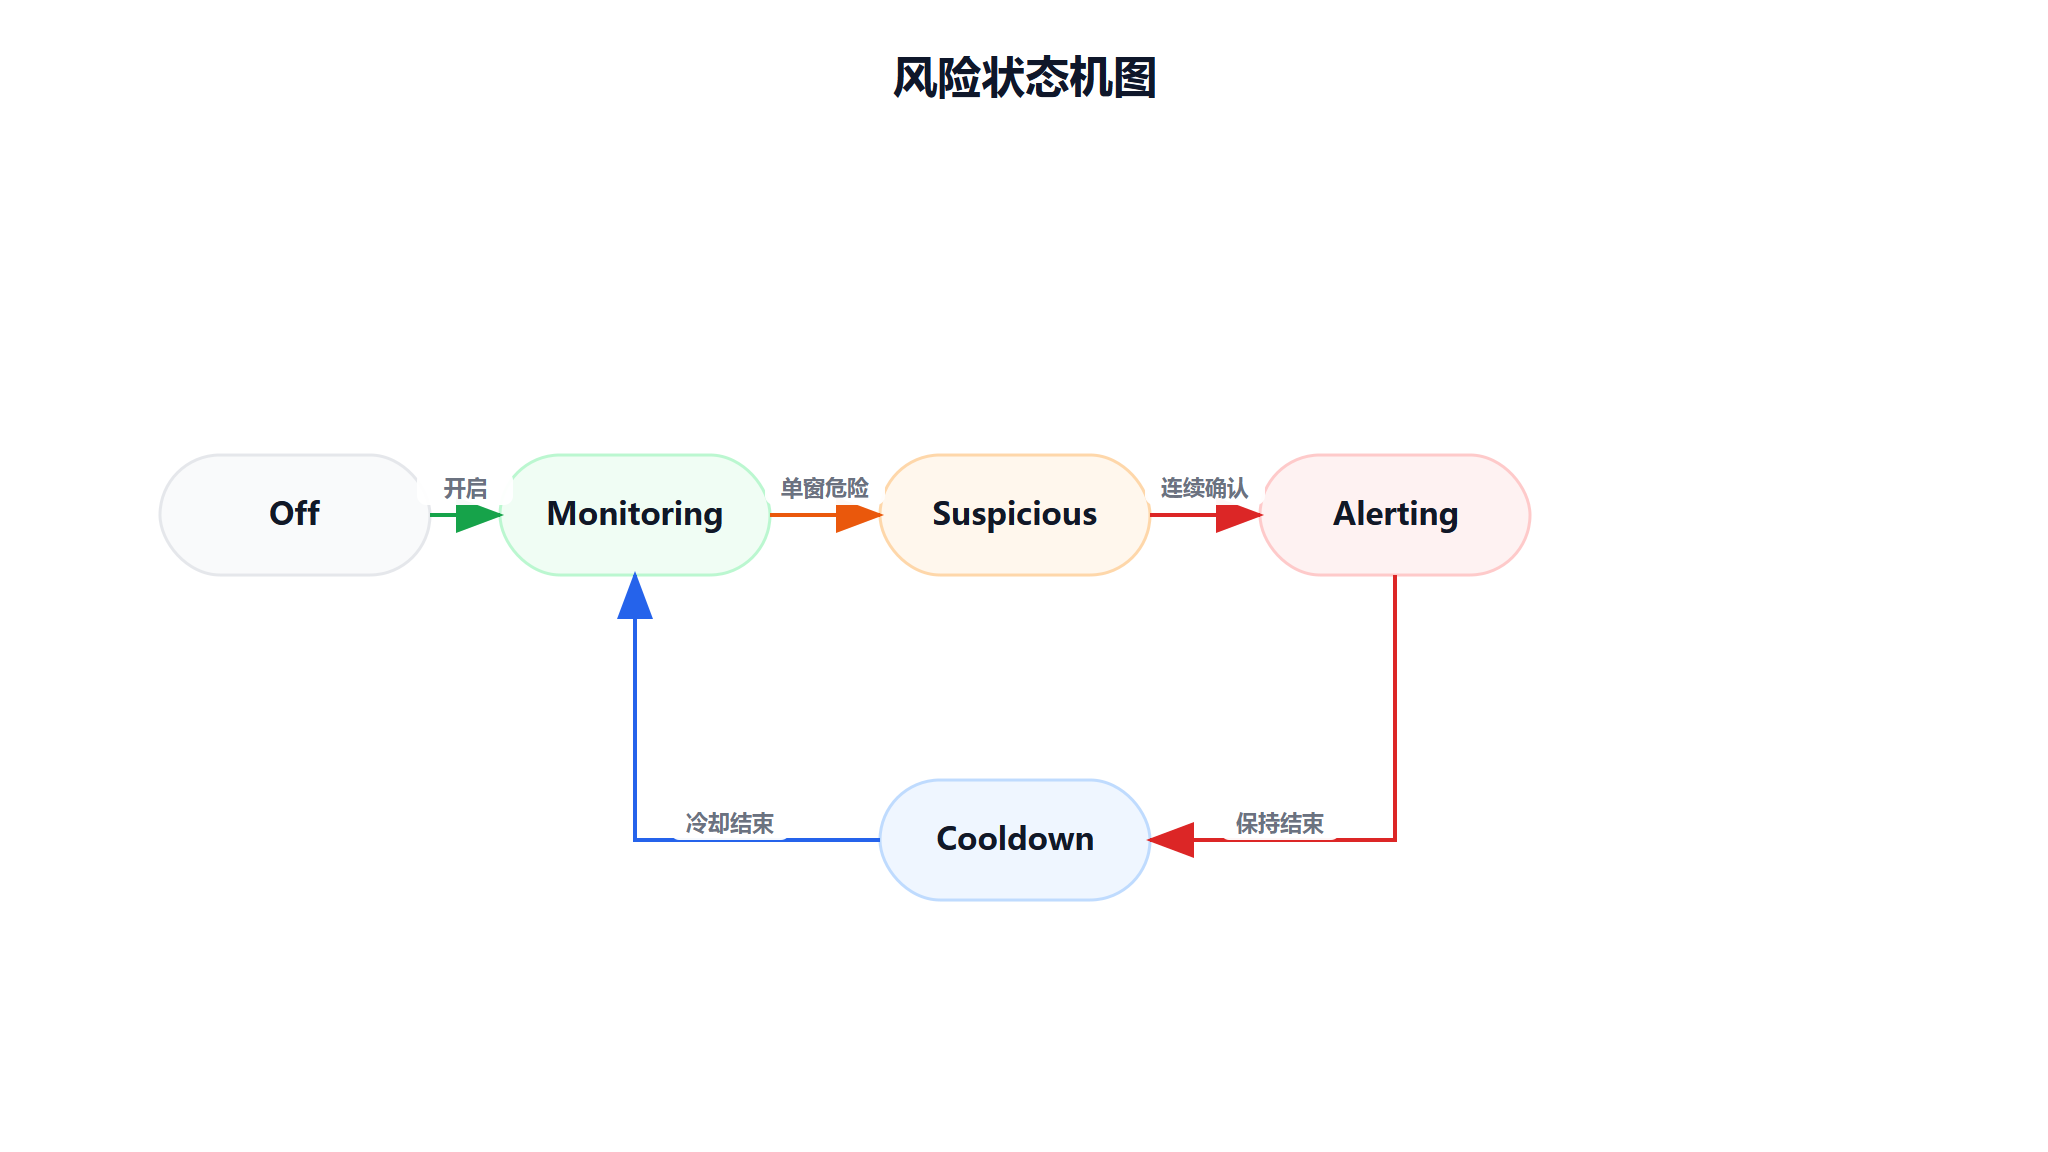
\includegraphics[width=0.95\linewidth]{figures/generated_diagrams/f04_risk_state_machine.png}
\caption{风险状态机图}
\end{figure}

\noindent{\small 状态迁移说明：Monitoring 表示持续监听，Suspicious 表示可疑风险，Alerting 表示危险告警，Cooldown 表示冷却抑制；系统通过连续确认进入告警，通过保持和冷却避免反复闪烁。}

\noindent\textbf{危险声分类决策逻辑。} 模型对每个音频窗口输出危险概率，但系统不直接将该概率作为提醒依据，而是通过风险融合层将其转化为稳定状态。表 \ref{tab:decision-logic} 给出各阶段的输入、判断依据和输出动作。

\begin{table}[htbp]
\centering
\caption{危险声分类与风险融合决策逻辑}
\label{tab:decision-logic}
\begin{tabularx}{\linewidth}{p{2.1cm}>{\RaggedRight\arraybackslash}p{2.8cm}>{\RaggedRight\arraybackslash}X>{\RaggedRight\arraybackslash}p{2.1cm}}
\toprule
阶段 & 输入 & 判断依据 & 输出动作 \\
\midrule
单窗推理 & PCM 音频窗口 & Fbank + ESP-DL 输出危险概率 & 原始概率 \\
连续确认 & 连续窗口概率序列 & 连续 $N$ 个窗口危险概率均高于阈值 & 触发可疑状态 \\
告警保持 & 可疑风险确认信号 & 达到最少告警保持时长，防止闪烁 & 进入危险告警 \\
冷却抑制 & 告警结束信号 & 环境安全后强制冷却，避免重复触发 & 进入冷却状态 \\
状态回退 & 新窗口概率低于阈值 & 证据不足时撤销可疑状态 & 回到监听状态 \\
\bottomrule
\end{tabularx}
\end{table}

\noindent\textbf{灵敏度、震动与低功耗安全监听。}

当前固件已经把听障辅助所需的三项工程能力接入主链路。第一，危险识别页提供保守、标准、敏感三档灵敏度，服务层分别映射为 0.95、0.90、0.85 的 ESP-DL 单窗危险阈值；每次切换档位都会重置后处理窗口计数，避免旧档位下的可疑证据影响新策略。第二，提醒层在新的危险事件产生时触发首次危险强震，震动任务独立运行，不阻塞推理回调和告警投递；当前节奏为 220ms 开、90ms 间隔、220ms 再开，并在退出前兜底关闭马达。第三，后台安全监听机制不再绑定危险识别页面，而是由后台服务统一维护；当用户开启安全监听且电源预算允许、麦克风未被前台音频占用、前台 ESP-DL 运行资源未被占用时，后台会话启动危险识别，反之暂停或恢复。

\noindent 这三项设计使作品从“能识别危险声音”进一步接近可穿戴产品：用户可按场景选择误报/漏报倾向，听障用户可通过触觉通道获得即时提醒，系统也能在电源和资源预算内协调安全监听、UI、网络与辅助交互。

\noindent\textbf{Hermes 任务辅助协同流程。}

Hermes 任务辅助流程是手表在安全提醒之外的协同能力。Hermes 是项目配套的个人 AI Agent 服务，适合承担长期记忆、任务理解、工具调用和跨设备协同；ESP32-S3 手表则作为随身交互与控制终端，负责语音/文本输入、状态显示和简短回执展示。用户按住手表说话或提交文本后，手表通过云服务端提交请求，服务器侧 ASR/Hermes 处理后返回结构化回执；用户离开电脑后，仍可在授权范围内通过 Hermes 联动电脑端工具执行文件整理、资料查询、日程管理和内容生成等事务，并在手表端接收回执、提醒和任务结果摘要。该设计让端侧安全提醒与日常任务辅助各自保持清晰分工，也使手表更符合随身可穿戴入口的产品定位。

\begin{figure}[htbp]
\centering
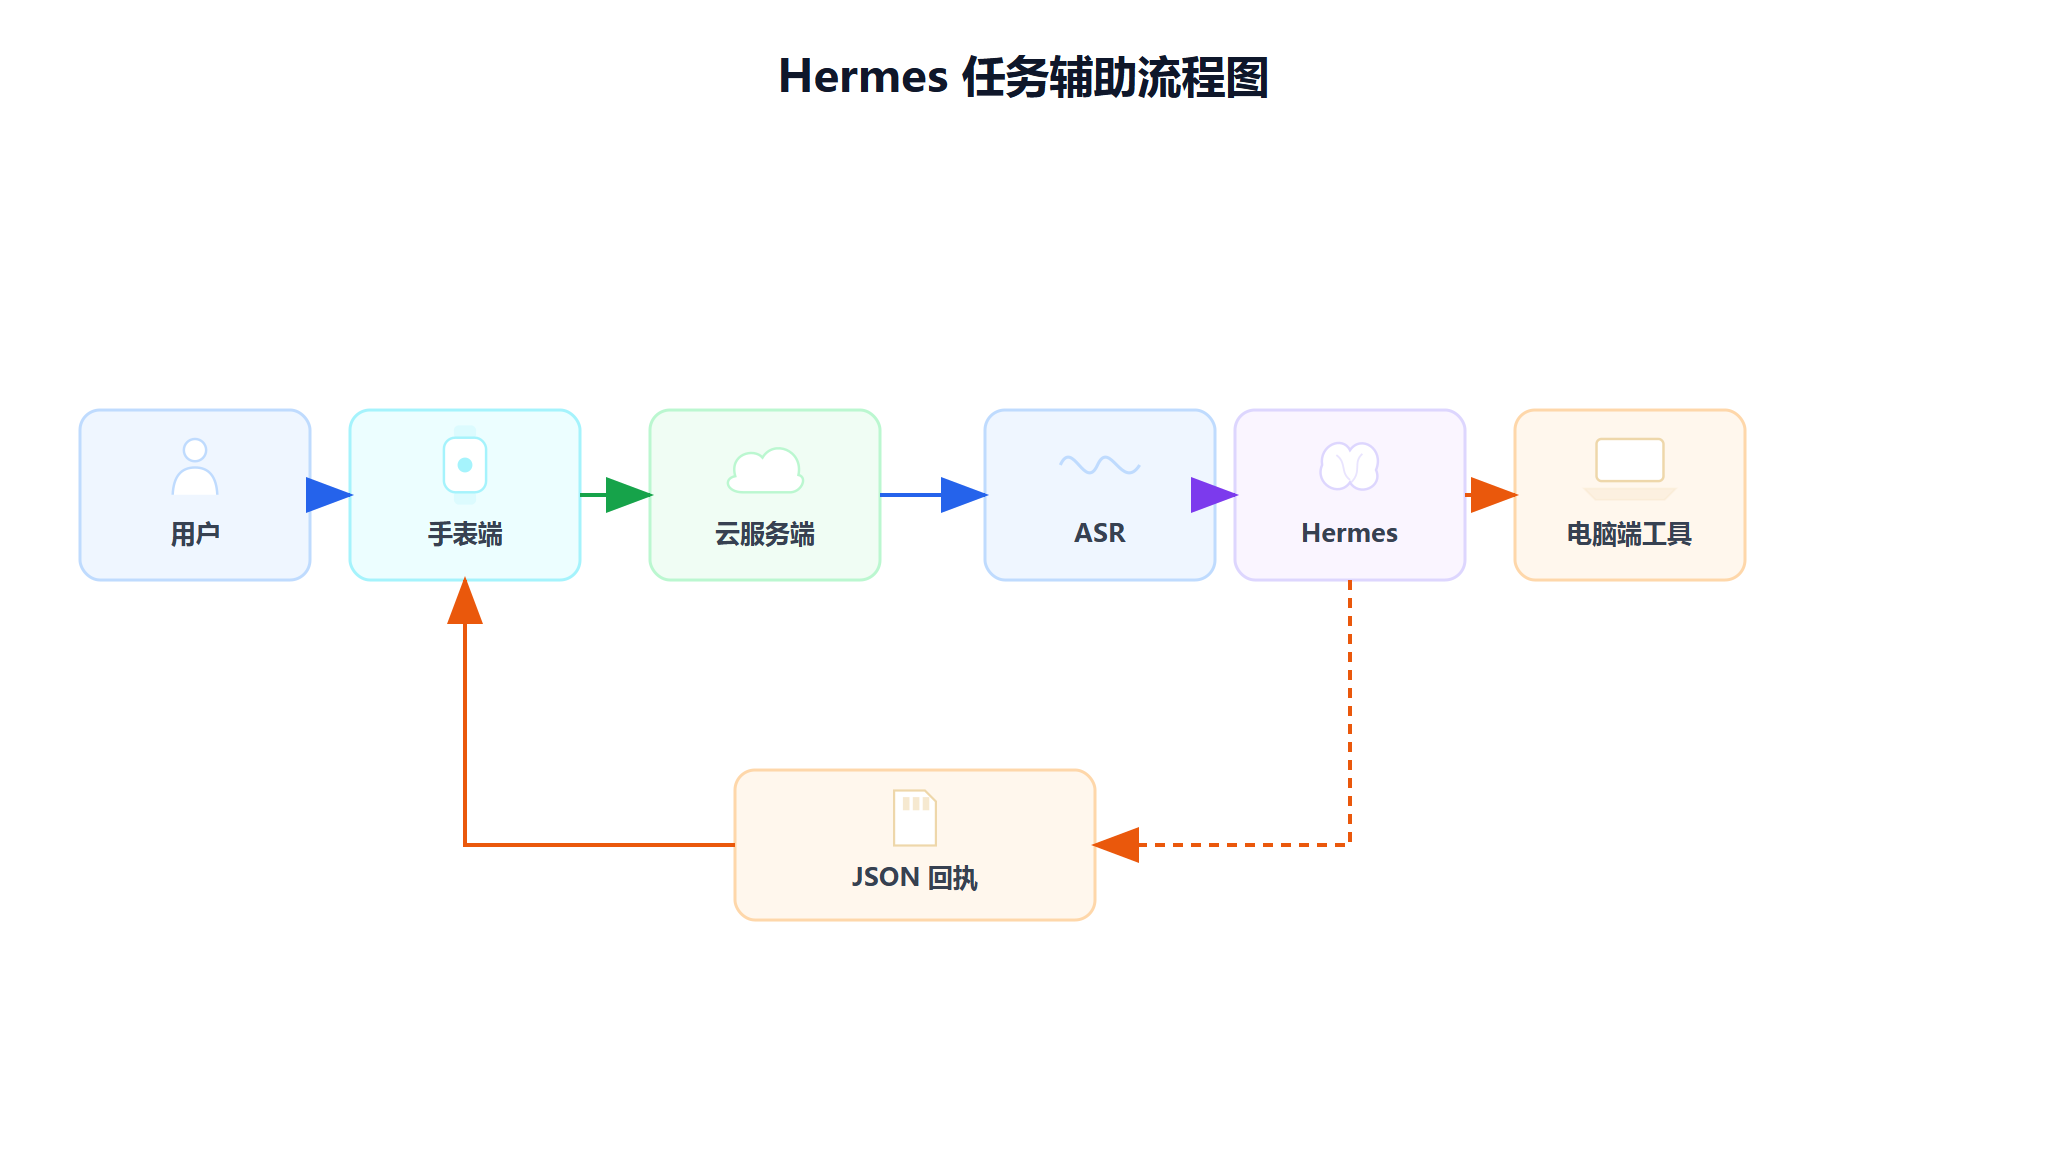
\includegraphics[width=0.95\linewidth]{figures/generated_diagrams/f05_hermes_flow.png}
\caption{Hermes 任务辅助协同流程图}
\end{figure}

\noindent\textbf{数据闭环与模型优化流程。}

系统的数据闭环采用“先本地保存，再离线分析”的路线，安全告警路径只负责本地采样与记录。手表端在识别过程中保留连续音频缓存；当风险状态机确认危险事件后，样本记录服务保存触发前后约 2 秒的音频片段，并写入 SD 卡 WAV 文件和 JSON 元数据。当前阶段已完成本地样本采集闭环，人工导出、离线标注和再训练作为后续模型优化路径。

\begin{figure}[htbp]
\centering
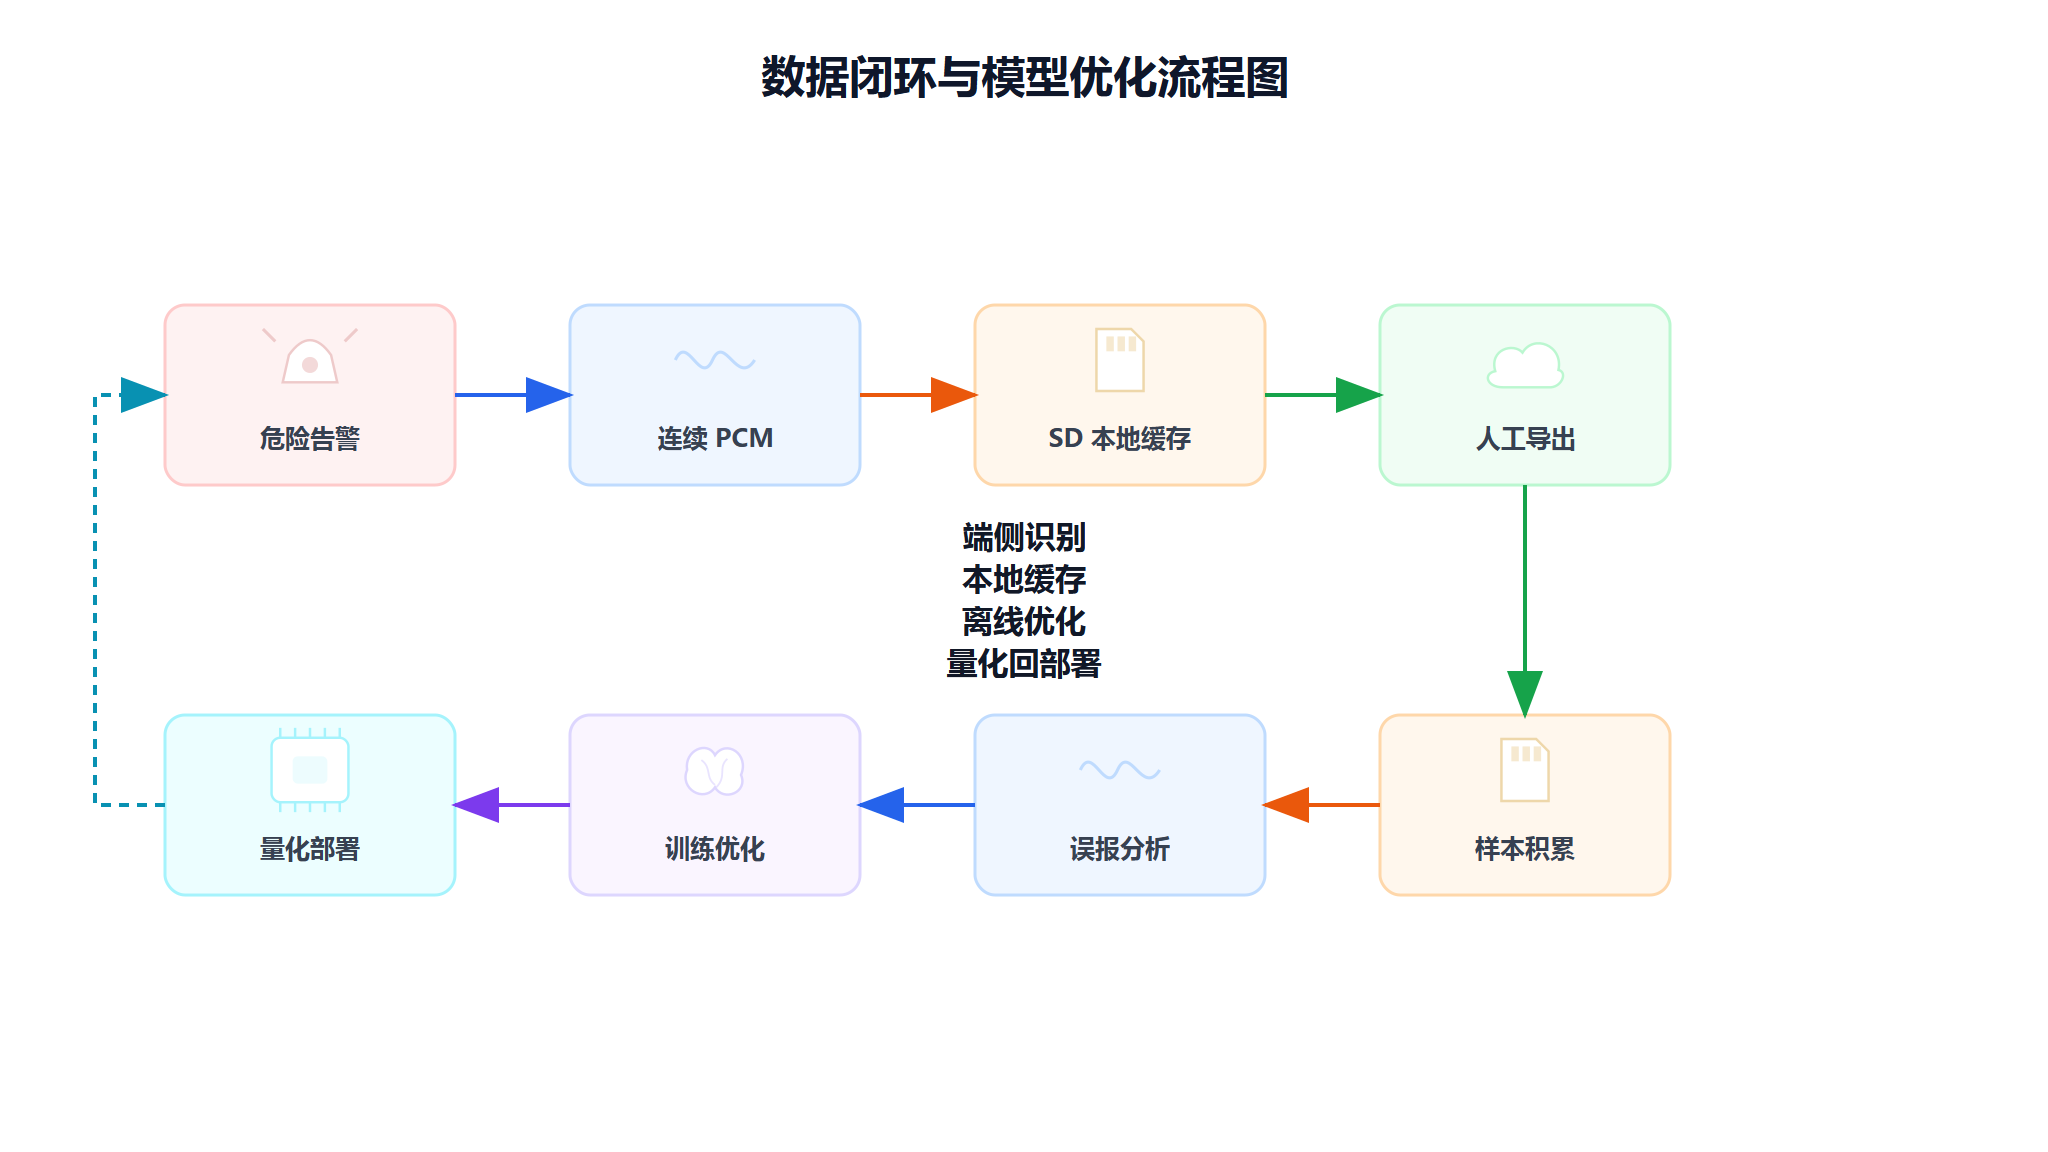
\includegraphics[width=0.95\linewidth]{figures/generated_diagrams/f06_data_loop.png}
\caption{数据闭环与模型优化流程图}
\end{figure}

当前仓库第一阶段已经完成本地样本保存语义：手表端可在危险触发时从本地音频缓存中截取前后片段，并由后台写入任务稳定保存到 SD 卡。后续优化阶段先以人工导出 SD 样本、离线标注、误报分析和训练集整理为主，不在本版报告中扩展为联网样本闭环。

\noindent\textbf{App 端远程补充告警方案。}

在远程补充告警链路上，当前实现采用“ESP32-S3 手表确认危险 -> 本地屏幕/震动提醒立即触发 -> 后台任务上报告警 -> 云服务端转发 -> App/手机通知栏提醒”的最小闭环。危险识别服务首次确认危险后，只在回调外投递一个轻量事件；告警投递服务通过 FreeRTOS 队列交给后台任务，由后台任务向云服务端发起 HTTPS 告警请求。服务器收到告警后再转发给 Android App 或手机通知栏。这样可以保证本地安全提醒不受网络状态影响，TLS 网络请求也不会阻塞 ESP-DL 音频推理路径。

\begin{figure}[htbp]
\centering
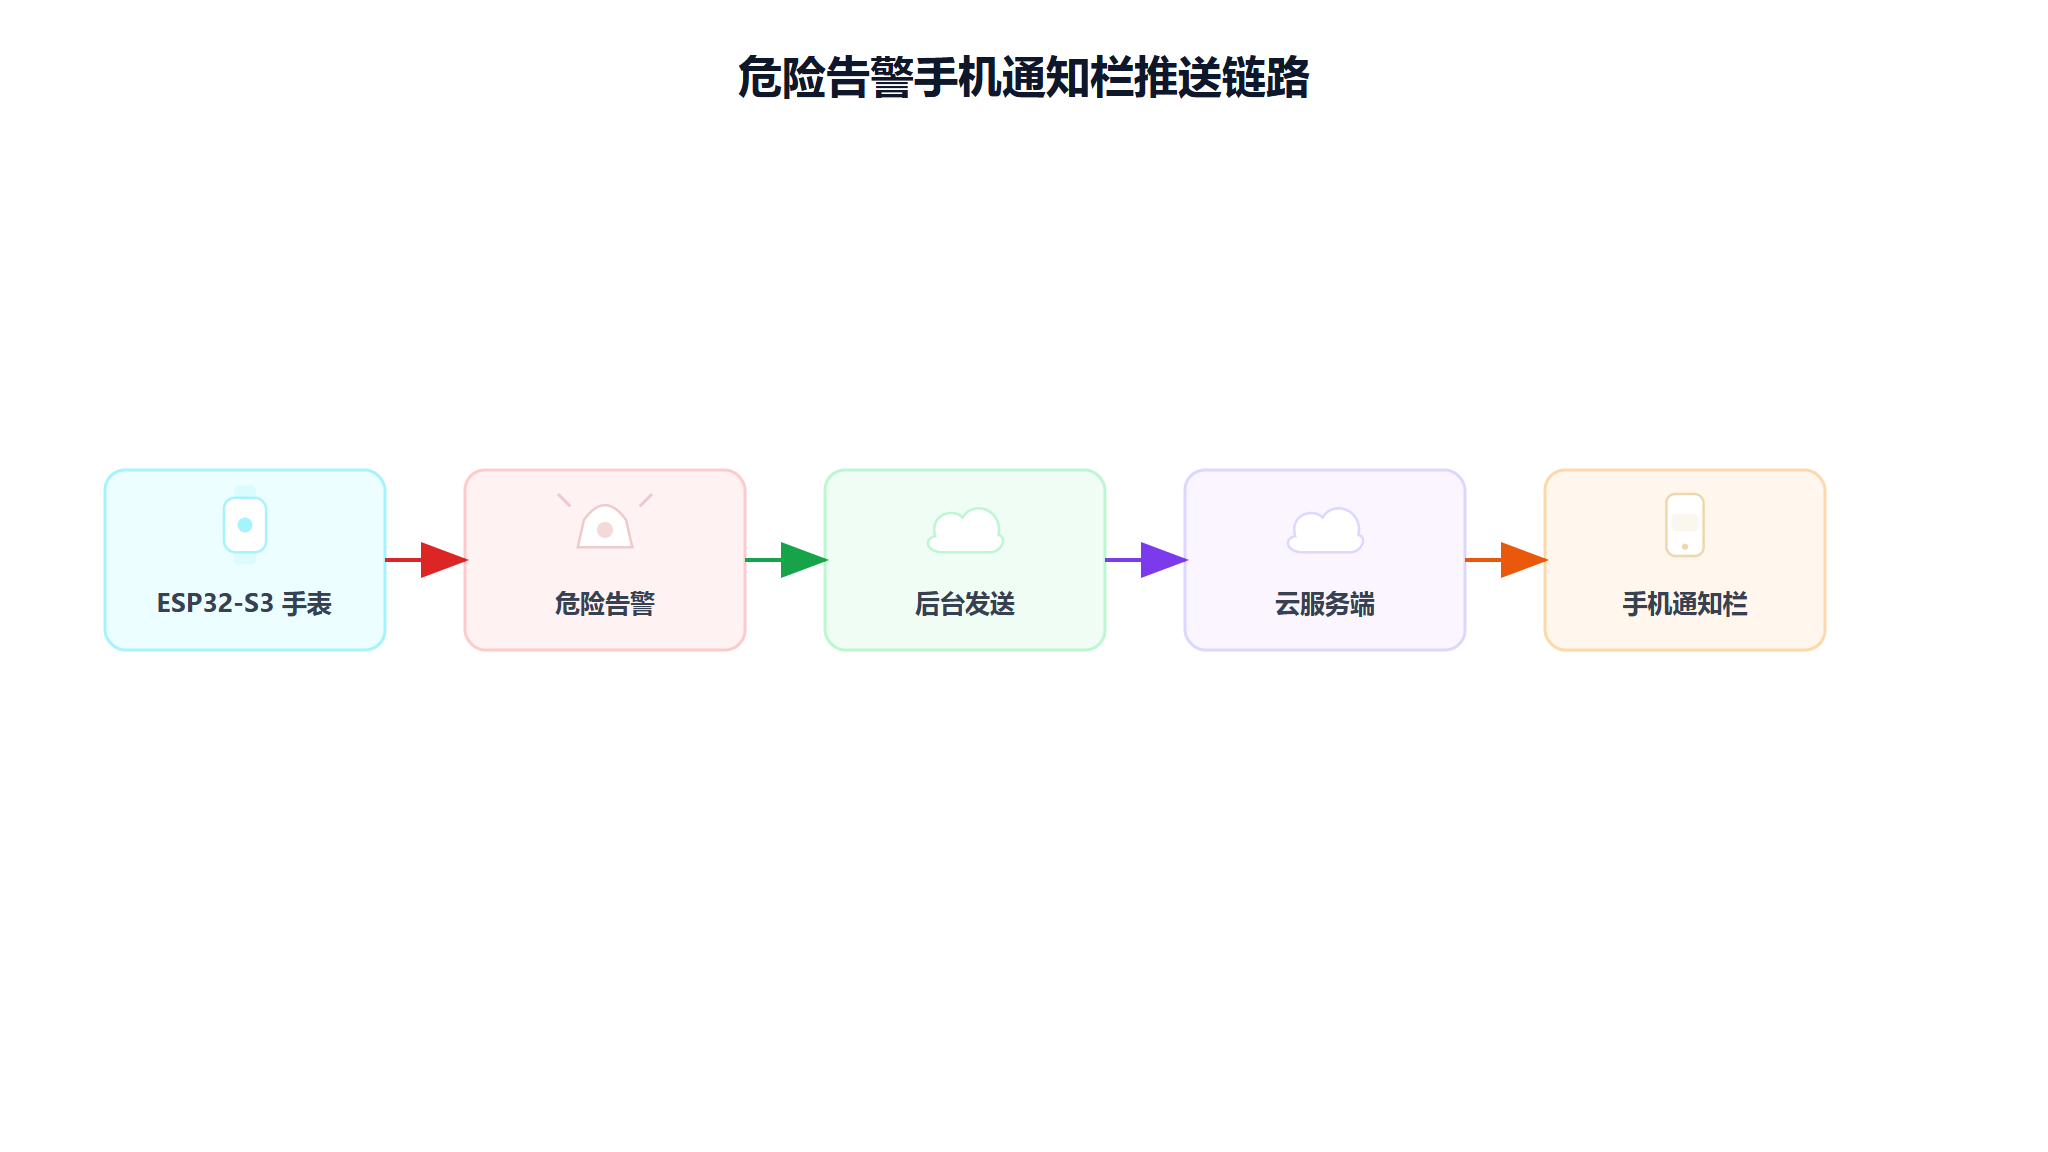
\includegraphics[width=0.95\linewidth]{figures/generated_diagrams/f12_phone_alert_chain.png}
\caption{危险告警 App/手机端远程补充告警链路}
\end{figure}

该方案的工程边界较清晰：危险识别服务只负责判断风险状态并投递事件；告警服务隔离危险识别与上层服务实现；后台任务负责带超时保护的 HTTPS 告警请求；本地提醒不依赖云端返回结果。当前已联调手机端远程提醒链路，家属或监护人绑定提醒可基于同一链路继续扩展。

\noindent\begin{tabularx}{\linewidth}{p{3.2cm}>{\RaggedRight\arraybackslash}X >{\RaggedRight\arraybackslash}p{4.0cm}}
\toprule
环节 & 作用 & 设计取舍 \\
\midrule
危险识别服务 & 首次确认危险后生成告警事件 & 不在推理回调中执行网络请求 \\
告警投递服务 & 校验网络状态并投递后台发送任务 & 网络失败不影响本地提醒 \\
后台发送任务 & 后台发送 HTTPS 告警请求到服务器 & 失败只记录日志，不影响本地安全提醒 \\
App/手机通知端 & 接收服务器推送并展示通知栏提醒 & 作为远程补充提醒，后续可面向绑定家属或监护人扩展 \\
\bottomrule
\end{tabularx}

\section*{第三部分\quad 完成情况及性能参数}
\addcontentsline{toc}{section}{第三部分 完成情况及性能参数}

本部分按“核心安全链路优先”的方式展示实现成果，重点呈现端侧推理、风险状态机、灵敏度档位、震动提醒、低功耗安全监听、本地样本保存和 App 端补充告警的验证记录。辅助交互能力单独列为扩展成果，避免削弱听障安全提醒和嵌入式边缘 AI 主线。

\subsection*{3.1 整体介绍}

当前项目已形成 ESP32-S3 固件、危险识别服务、风险状态机、三档灵敏度、震动提醒、后台安全监听、App/手机端远程补充告警、SD 危险样本保存和云服务端接口契约等基础模块。Hermes 手表页面作为辅助交互模块保留，用于展示手表作为残障用户随身任务辅助与回执接收入口的扩展价值。报告中的成果证明以串口日志、模型文件、状态机流转、源码测试、构建结果、真机现象和接口联调记录为主。

\placeholderfig{整机实物组图：正面、斜 45 度、佩戴或装配状态合成一张，使用匿名真实照片}

\subsection*{3.2 工程成果}

\subsubsection*{3.2.1 机械成果}

机械成果方面，当前 PCB 板框已经完成，尺寸为 46.0 mm $\times$ 37.0 mm，并预留 5 个 $\Phi$1.8 mm 定位孔、USB Type-C 避让口和左右圆角外形，能够与手表表壳和佩戴结构配合。该部分证明作品不是只停留在软件仿真，而是已经围绕可穿戴终端完成了板级机械边界设计；整机实物组图集中展示正面、斜 45 度和佩戴/装配状态。

\subsubsection*{3.2.2 电路成果}

电路成果方面，系统已经完成主控、电源、传感器、音频、显示触摸、通信存储和提醒通道的原理图与 PCB 布局设计。图 \ref{fig:system-schematic} 展示了各模块的完整连接关系，图 \ref{fig:pcb-layout} 展示了顶层和底层布局。对比赛报告而言，这组硬件图能够证明 ESP32-S3、双麦克风、音频 ADC、屏幕触摸、电源管理、SD 存储和马达提醒均已纳入同一块手表主板设计，为端侧 AI 安全提醒提供硬件落点。

\placeholderfig{PCB 实物组图：PCB 正面、背面、上电或焊接调试状态合成一张，使用匿名真实照片}

\clearpage

\subsubsection*{3.2.3 软件成果}

\noindent\begin{tabularx}{\linewidth}{p{3.2cm}>{\RaggedRight\arraybackslash}X >{\RaggedRight\arraybackslash}p{4.2cm}}
\toprule
成果类别 & 当前内容 & 证据状态 \\
\midrule
端侧推理 & ESP-DL 推理组件、音频处理模块、模型加载与推理模块 & 板端运行日志与模型文件记录 \\
风险融合 & 连续确认、告警保持、冷却和状态快照 & 状态机完整流转日志 \\
灵敏度档位 & 保守/标准/敏感三档，映射 0.95/0.90/0.85 阈值 & 服务层与 UI 事件代码已实现 \\
本地提醒界面 & 展示监听、危险提醒、档位和状态变化 & 危险告警/震动组图作为成果证据 \\
震动提醒 & 首次确认危险后由独立后台任务驱动马达短促强震 & 与危险告警/震动组图共同展示 \\
后台安全监听 & 后台会话按电源预算、麦克风占用和前台运行资源启停 & 灵敏度与后台安全监听截图作为成果证据 \\
App 远程补充告警 & 确认危险后通过后台任务向云服务端上报，再推送到 App/手机通知栏 & App/手机通知链路组图作为成果证据 \\
危险样本保存 & 确认危险后保存前 1 s + 后 1 s WAV/JSON 到 SD 卡 & 源码测试、完整构建和串口真机测试已通过 \\
安全边界 & 云端密钥不下发设备端，手表通过设备鉴权机制访问受控云服务接口 & 接口契约与鉴权测试记录 \\
Hermes 任务辅助 & 支持语音/文本任务记录、提醒创建、回执展示和授权范围内的电脑端事务协同 & Hermes 回执截图作为辅助证据 \\
\bottomrule
\end{tabularx}

\clearpage

\subsection*{3.3 特性成果}

本作品的特性成果围绕“端侧识别、本地提醒、远程补充、样本闭环”展开。核心安全能力均在手表端完成，网络与 Hermes 仅作为补充服务；因此本节先呈现安全闭环和模型部署结果，再说明 App 端补充告警、SD 样本保存和 Hermes 辅助回执。

{\small
\setlength{\tabcolsep}{4pt}
\noindent\begin{longtable}{p{3.1cm}>{\RaggedRight\arraybackslash}p{4.0cm}>{\RaggedRight\arraybackslash}p{6.0cm}}
\toprule
特性类别 & 验证方式 & 完成结果 \\
\midrule
端侧危险声识别 & 播放鸣笛、警笛样本并观察手表状态 & 手表可在本地完成危险判断，首次危险判断到告警约 380--400 ms。 \\
本地风险状态机 & 连续输入危险/安全音频窗口 & 已完成监听、可疑、告警、冷却状态迁移；危险结束后可回到监听状态。 \\
屏幕与震动提醒 & 触发危险告警并观察界面和马达反馈 & 高对比危险界面与短促强震已接入提醒管理服务，断网时仍可触发本地提醒。 \\
灵敏度档位 & 在危险识别页切换保守、标准、敏感三档 & 三档阈值分别为 0.95、0.90、0.85，切换后会重置后处理计数。 \\
后台安全监听 & 开启安全监听后切换页面和资源占用状态 & 后台可按电源预算、麦克风占用和前台运行资源启动、暂停或恢复危险识别；24 h 连续运行未出现崩溃、看门狗复位或内存耗尽。 \\
SD 本地样本保存 & 触发危险告警后检查 SD 卡文件 & 已写出触发前后约 2 s、16 kHz 单声道 WAV 与 JSON 元数据。 \\
App 远程补充告警 & 手表触发危险事件，经云服务端转发 & 手机端通知链路已完成联调，服务器端鉴权、去重、超时和脱敏测试通过；家属或监护人接收提醒可基于同一链路扩展。 \\
Hermes 任务辅助 & 手表提交文本或语音任务 & 手表端可显示简短回执和任务结果摘要，电脑端工具协同具备后续扩展基础。 \\
\bottomrule
\end{longtable}
}

\noindent\textbf{端侧识别与本地提醒闭环。}

端侧危险声识别链路已经形成从麦克风采集、Fbank 特征提取、ESP-DL 推理、连续证据融合到本地提醒的闭环。危险声触发后，状态机会从监听进入可疑，再确认危险告警；危险结束后进入冷却并恢复监听。该链路不依赖网络，网络异常只影响远程补充告警，不影响手表端屏幕和震动提醒。

相关状态机日志可并入危险告警/震动组图，与危险提醒界面和震动关键帧共同作为核心证据。

\placeholderfig{危险告警/震动组图：危险提醒界面、状态机日志片段、震动短视频关键帧合成一张}

\noindent\textbf{模型效果与板端资源。}

模型训练与离线评估在 PC 端完成，训练仓库为 AudioClassification-Pytorch，深度学习框架为 PyTorch，训练/评估脚本使用 Python 编写。CUDA 仅用于训练与评估加速，本次验证使用 NVIDIA GeForce RTX 5060，PyTorch 版本为 \texttt{torch 2.10.0+cu130}。上述环境仅用于模型训练、评估和导出，手表端不运行 PyTorch；端侧实际部署平台为 ESP32-S3，推理框架为 ESP-DL。

当前部署模型为基于 DSCNNTiny 的二分类危险声识别模型，输入为 1 s、16 kHz 单声道音频，经 Fbank 提取为约 98 帧、40 mel bins 的二维特征后，输出 non-danger / danger 二分类结果。模型以 \texttt{.espdl} 格式部署到 ESP32-S3，并通过 ESP-DL int8 推理运行。主要指标如下：

{\small
\setlength{\tabcolsep}{4pt}
\noindent\begin{longtable}{p{3.0cm}>{\RaggedRight\arraybackslash}p{4.0cm}>{\RaggedRight\arraybackslash}p{6.0cm}}
\toprule
类别 & 指标 & 结果 \\
\midrule
模型输入 & 音频与特征 & 1 s、16 kHz、单声道；Fbank，40 mel bins，约 98 frames。 \\
模型结构 & 网络与输出 & DSCNNTiny；non-danger / danger 二分类；部署阈值 0.90。 \\
部署方式 & 端侧格式 & \texttt{.espdl} 文件，ESP-DL int8 推理，模型大小约 31.4 KB。 \\
离线评估 & 测试范围 & 131 条 edge 测试集，覆盖 background、horn、siren。 \\
离线评估 & 综合指标 & Accuracy 96.18\%，Recall 93.83\%，误报率 0.00\%，Precision 100.00\%，F1-score 96.82\%。 \\
混淆矩阵 & 二分类统计 & TN=50，FP=0，FN=5，TP=76。 \\
来源类别 & 分类结果 & background 50/50 正确；horn 39/41 正确；siren 37/40 正确。 \\
板端资源 & 内存与存储 & 内部 RAM 5,616 B，PSRAM 272,680 B，Flash 32,144 B。 \\
板端耗时 & 单窗处理 & Fbank 平均 32.66 ms，模型推理平均 53.41 ms，合计平均 86.07 ms。 \\
\bottomrule
\end{longtable}
}

\noindent\textbf{灵敏度、震动与后台安全监听。}

当前危险识别服务提供保守、标准、敏感三档策略：保守模式阈值 0.95，标准模式阈值 0.90，敏感模式阈值 0.85，三档均保持 2 个连续危险窗口确认、3 个连续安全窗口清除、2000 ms 告警保持和 3000 ms 冷却。危险识别页切换档位后，服务层会更新阈值、重置后处理计数，并同步到 ESP-DL 推理链路。

本地提醒方面，提醒管理服务在新的危险告警产生后同时拉起屏幕危险覆盖层、一次性提示音和短促强震。震动播放由独立 FreeRTOS 任务执行，避免在推理回调或提醒编排路径中阻塞；任务退出前会兜底关闭马达，降低异常路径下马达长时间保持开启的风险。低功耗安全监听方面，后台服务会综合电源预算、麦克风占用和前台运行资源，统一启动、停止或恢复危险识别会话。该设计使安全监听不依赖危险识别页面是否可见，也不会在前台语音交互或维护窗口中强抢资源。

\placeholderfig{灵敏度与后台安全监听截图：同图展示保守/标准/敏感三档、安全监听开关，可在角落合并 24 h 稳定运行日志摘要}

\noindent\textbf{危险样本 SD 保存闭环。}

危险样本闭环已经从“后续设想”推进到本地保存阶段。手表端在识别过程中维护连续音频缓存；当风险状态机确认危险事件后，样本记录模块会保存触发前 1 秒和触发后 1 秒的音频片段，最终在 SD 卡下写入 WAV 与 JSON 元数据。JSON 中包含置信度、采样率、声道数和前后采样时长等信息，便于本地复盘、人工筛选和离线标注。

该链路已经通过源码测试、完整构建和串口真机测试验证。在板端测试中，系统可在不依赖网络和远程通知的条件下生成 16 kHz 单声道音频样本，并写出 WAV 与同名 JSON 元数据。SD 样本保存组图应同时展示成对生成的 WAV/JSON 文件和 JSON 中的置信度、采样率、声道数、前后采样时长等关键字段。

\placeholderfig{SD 样本保存组图：SD 目录中的 WAV/JSON 文件与打开后的 JSON 关键字段合成一张}

\noindent\textbf{App/手机端远程补充告警联调。}

App/手机端远程补充告警链路的定位是“本地提醒优先、远程获知补充”：手表端首次确认危险后，先立即触发本地屏幕提醒和震动提醒，再通过告警投递接口提交危险事件，由 FreeRTOS 队列交给后台发送任务，向云服务端发起带超时保护的 HTTPS 告警请求，服务器再将告警送达 Android App 或手机通知栏。危险识别回调不直接执行 TLS 请求，网络失败、云端接口未配置或队列忙只记录跳过，不影响本地屏幕/震动提醒安全闭环。

联调记录显示该链路已经完成真机验证：危险告警事件可通过 HTTPS 告警请求到达云服务端，并触发 App/手机通知栏提醒；服务器侧已启用设备鉴权，未授权请求会被拒绝，合法请求返回成功响应。当前复测中，固件侧 ESP-DL、危险检测、SD 样本保存和云服务接口相关源码测试共 30 项通过；服务器端接口测试共 42 项通过，覆盖语音/文本回执、告警鉴权、请求去重、超时和敏感信息脱敏。App/手机通知链路组图集中展示手表危险告警画面、App/手机通知栏截图和云服务端告警接收日志。该链路可进一步支持绑定家属或监护人接收远程提醒。

\placeholderfig{App/手机通知链路组图：手表触发危险、App/手机通知栏、云服务端接收日志合成一张；家属或监护人绑定提醒后续扩展}

\noindent\textbf{Hermes 任务辅助回执。}

Hermes 链路作为辅助交互扩展进行验证。手表端可向 Hermes 提交文本或语音任务，云服务端完成任务记录、语音识别和结构化回执，手表端再展示简短结果摘要。当前已完成语音/文本任务提交与手表端回执展示，电脑端工具协同具备后续扩展基础。该能力使手表具备残障用户随身任务辅助与信息回执入口。

\placeholderfig{Hermes 回执截图：手表端请求与回执摘要合成一张}

\section*{第四部分\quad 总结}
\addcontentsline{toc}{section}{第四部分 总结}

\subsection*{4.1 可扩展之处}

后续工作可从五个方向继续完善：一是增强危险声模型的抗噪能力，补充中文大声人声、电视外放、衣物摩擦、公交地铁等易误报负样本，降低误报；二是在已完成首次强震和三档灵敏度的基础上，继续完善持续提醒节奏、用户通知模式和事件回顾；三是补齐 App/手机端远程补充告警的告警历史、断线状态提示、电池优化白名单说明和家属/监护人绑定提醒；四是把 SD 本地样本采集扩展为人工导出、离线标注、误报分析和模型再训练流程；五是在已有后台安全监听资源门控基础上继续量化功耗，完善安全监听、网络服务、屏幕刷新和辅助交互的可穿戴功耗预算。Hermes 可继续完善长期记忆、陪伴式交互和电脑端工具联动等能力。

\subsection*{4.2 心得体会}

本作品的研发过程表明，嵌入式 AI 作品不能只停留在模型推理成功，还必须把模型输出接入稳定的工程状态、用户可感知的提醒方式和可验证的测试证据。对于听障辅助场景，真正重要的不是显示一个分类标签，而是让用户在合适时间收到可信、低打扰的提醒。

当前作品已经形成端侧识别、风险融合、震动与屏幕本地提醒、灵敏度档位、后台安全监听、App/手机端远程补充告警和本地样本保存的工程闭环。报告中可验证的核心证据包括模型大小、推理耗时、状态机流转、连续运行日志、灵敏度与震动实现、云服务端鉴权与请求去重测试、App/手机端告警联调记录，以及 SD 样本保存的源码测试和串口真机测试；这些证据共同说明作品不是单纯的概念方案，而是已经落到 ESP32-S3 手表端的边缘 AI 应用。

同时，手表与 Hermes 的端云分工体现了嵌入式系统设计中的边界意识。ESP32-S3 适合承担随身输入、端侧识别、状态显示和轻量请求，用户离开电脑后仍能通过手表把任务交给 Hermes 并接收回执；长期记忆、复杂任务整理、任务执行和跨设备工具调用则更适合放到 Hermes 与服务器端。这样的分工使本地安全链路保持轻量稳定，也让面向残障用户的任务辅助和陪伴式交互能力自然接入。

\section*{第五部分\quad 参考文献}
\addcontentsline{toc}{section}{第五部分 参考文献}

\begin{enumerate}
  \item 全国大学生嵌入式芯片与系统设计竞赛官网，应用赛道作品上传要求。
  \item 2026 年全国大学生嵌入式芯片与系统设计竞赛应用赛道作品报告模板。
  \item Espressif Systems. ESP32-S3 技术参考手册与 ESP-IDF 编程指南。
  \item Espressif Systems. ESP-DL 官方文档。
  \item LVGL 官方文档。
  \item WHO 或 NIDCD 关于听力损失和辅助设备的公开资料。
\end{enumerate}

\end{document}
